% ####################################################################
% Basic configuration of Beamera class and Jagiellonian theme
% ####################################################################
\RequirePackage[l2tabu, orthodox]{nag}



\ifx\PresentationStyle\notset
  \def\PresentationStyle{dark}
\fi



% Options: t - align frame text to the top.
\documentclass[10pt,t]{beamer}
\mode<presentation>
\usetheme[style=\PresentationStyle]{jagiellonian}




% ------------------------------------------------------------------------------------
% Procesing configuration files of Jagiellonian theme located
% in the directory "preambule"
% ------------------------------------------------------------------------------------
% Configuration for polish language
% Need description
\usepackage[polish]{babel}
% Need description
\usepackage[MeX]{polski}



% ------------------------------
% Better support of polish chars in technical parts of PDF
% ------------------------------
\hypersetup{pdfencoding=auto,psdextra}

% Package "textpos" give as enviroment "textblock" which is very usefull in
% arranging text on slides.

% This is standard configuration of "textpos"
\usepackage[overlay,absolute]{textpos}

% If you need to see bounds of "textblock's" comment line above and uncomment
% one below.

% Caution! When showboxes option is on significant ammunt of space is add
% to the top of textblock and as such, everyting put in them gone down.
% We need to check how to remove this bug.

% \usepackage[showboxes,overlay,absolute]{textpos}



% Setting scale length for package "textpos"
\setlength{\TPHorizModule}{10mm}
\setlength{\TPVertModule}{\TPHorizModule}


% ---------------------------------------
% Packages written for lectures "Geometria 3D dla twórców gier wideo"
% ---------------------------------------
% \usepackage{./Geometry3DPackages/Geometry3D}
% \usepackage{./Geometry3DPackages/Geometry3DIndices}
% \usepackage{./Geometry3DPackages/Geometry3DTikZStyle}
% \usepackage{./ProgramowanieSymulacjiFizykiPaczki/ProgramowanieSymulacjiFizykiTikZStyle}
% \usepackage{./Geometry3DPackages/mathcommands}


% ---------------------------------------
% Importing TikZ's libraries
% ---------------------------------------
\usetikzlibrary{arrows.meta}
\usetikzlibrary{positioning}





% % Configuration package "bm" that need for making bold symbols
\newcommand{\bmmax}{0}
\newcommand{\hmmax}{0}
\usepackage{bm}




% ---------------------------------------
% Packages for scientific texts
% ---------------------------------------
% \let\lll\undefined  % Sometimes you must use this line to allow
% "amsmath" package to works with packages with packages for polish
% languge imported
% /preambul/LanguageSettings/JagiellonianPolishLanguageSettings.tex.
% This comments (probably) removes polish letter Ł.
\usepackage{amsmath}  % Packages from American Mathematical Society (AMS)
\usepackage{amssymb}
\usepackage{amscd}
\usepackage{amsthm}
\usepackage{siunitx}  % Package for typsetting SI units.
\usepackage{upgreek}  % Better looking greek letters.
% Example of using upgreek: pi = \uppi


\usepackage{calrsfs}  % Zmienia czcionkę kaligraficzną w \mathcal
% na ładniejszą. Może w innych miejscach robi to samo, ale o tym nic
% nie wiem.







% !!!!!!!!!!!!!!!!!!!!!!!!!!!!!!
% !!!!!!!!!!!!!!!!!!!!!!!!!!!!!!
% EVIL STUFF
\if\JUlogotitle1
\edef\LogoJUPath{LogoJU_\JUlogoLang/LogoJU_\JUlogoShape_\JUlogoColor.pdf}
\titlegraphic{\hfill\includegraphics[scale=0.22]
{./JagiellonianPictures/\LogoJUPath}}
\fi

% ---------------------------------------
% Commands for handling colors
% ---------------------------------------


% Command for setting normal text color for some text in math modestyle
% Text color depend on used style of Jagiellonian

% Beamer version of command
\newcommand{\TextWithNormalTextColor}[1]{%
  {\color{jNormalTextFGColor}
    \setbeamercolor{math text}{fg=jNormalTextFGColor} {#1}}
}

% Article and similar classes version of command
% \newcommand{\TextWithNormalTextColor}[1]{%
%   {\color{jNormalTextsFGColor} {#1}}
% }



% Beamer version of command
\newcommand{\NormalTextInMathMode}[1]{%
  {\color{jNormalTextFGColor}
    \setbeamercolor{math text}{fg=jNormalTextFGColor} \text{#1}}
}


% Article and similar classes version of command
% \newcommand{\NormalTextInMathMode}[1]{%
%   {\color{jNormalTextsFGColor} \text{#1}}
% }




% Command that sets color of some mathematical text to the same color
% that has normal text in header (?)

% Beamer version of the command
\newcommand{\MathTextFrametitleFGColor}[1]{%
  {\color{jFrametitleFGColor}
    \setbeamercolor{math text}{fg=jFrametitleFGColor} #1}
}

% Article and similar classes version of the command
% \newcommand{\MathTextWhiteColor}[1]{{\color{jFrametitleFGColor} #1}}





% Command for setting color of alert text for some text in math modestyle

% Beamer version of the command
\newcommand{\MathTextAlertColor}[1]{%
  {\color{jOrange} \setbeamercolor{math text}{fg=jOrange} #1}
}

% Article and similar classes version of the command
% \newcommand{\MathTextAlertColor}[1]{{\color{jOrange} #1}}





% Command that allow you to sets chosen color as the color of some text into
% math mode. Due to some nuances in the way that Beamer handle colors
% it not work in all cases. We hope that in the future we will improve it.

% Beamer version of the command
\newcommand{\SetMathTextColor}[2]{%
  {\color{#1} \setbeamercolor{math text}{fg=#1} #2}
}


% Article and similar classes version of the command
% \newcommand{\SetMathTextColor}[2]{{\color{#1} #2}}










% ---------------------------------------
% Commands for few special slides
% ---------------------------------------
\newcommand{\EndingSlide}[1]{%
  \begin{frame}[standout]

    \begingroup

    \color{jFrametitleFGColor}

    #1

    \endgroup

  \end{frame}
}










% ---------------------------------------
% Commands for setting background pictures for some slides
% ---------------------------------------
\newcommand{\TitleBackgroundPicture}
{./JagiellonianPictures/Backgrounds/LajkonikDark.png}
\newcommand{\SectionBackgroundPicture}
{./JagiellonianPictures/Backgrounds/LajkonikLight.png}



\newcommand{\TitleSlideWithPicture}{%
  \begingroup

  \usebackgroundtemplate{%
    \includegraphics[height=\paperheight]{\TitleBackgroundPicture}}

  \maketitle

  \endgroup
}





\newcommand{\SectionSlideWithPicture}[1]{%
  \begingroup

  \usebackgroundtemplate{%
    \includegraphics[height=\paperheight]{\SectionBackgroundPicture}}

  \setbeamercolor{titlelike}{fg=normal text.fg}

  \section{#1}

  \endgroup
}










% ---------------------------------------
% Commands for lectures "Geometria 3D dla twórców gier wideo"
% Polish version
% ---------------------------------------
% Komendy teraz wykomentowane były potrzebne, gdy loga były na niebieskim
% tle, nie na białym. A są na białym bo tego chcieli w biurze projektu.
% \newcommand{\FundingLogoWhitePicturePL}
% {./PresentationPictures/CommonPictures/logotypFundusze_biale_bez_tla2.pdf}
\newcommand{\FundingLogoColorPicturePL}
{./PresentationPictures/CommonPictures/European_Funds_color_PL.pdf}
% \newcommand{\EULogoWhitePicturePL}
% {./PresentationPictures/CommonPictures/logotypUE_biale_bez_tla2.pdf}
\newcommand{\EUSocialFundLogoColorPicturePL}
{./PresentationPictures/CommonPictures/EU_Social_Fund_color_PL.pdf}
% \newcommand{\ZintegrUJLogoWhitePicturePL}
% {./PresentationPictures/CommonPictures/zintegruj-logo-white.pdf}
\newcommand{\ZintegrUJLogoColorPicturePL}
{./PresentationPictures/CommonPictures/ZintegrUJ_color.pdf}
\newcommand{\JULogoColorPicturePL}
{./JagiellonianPictures/LogoJU_PL/LogoJU_A_color.pdf}





\newcommand{\GeometryThreeDSpecialBeginningSlidePL}{%
  \begin{frame}[standout]

    \begin{textblock}{11}(1,0.7)

      \begin{flushleft}

        \mdseries

        \footnotesize

        \color{jFrametitleFGColor}

        Materiał powstał w ramach projektu współfinansowanego ze środków
        Unii Europejskiej w ramach Europejskiego Funduszu Społecznego
        POWR.03.05.00-00-Z309/17-00.

      \end{flushleft}

    \end{textblock}





    \begin{textblock}{10}(0,2.2)

      \tikz \fill[color=jBackgroundStyleLight] (0,0) rectangle (12.8,-1.5);

    \end{textblock}


    \begin{textblock}{3.2}(1,2.45)

      \includegraphics[scale=0.3]{\FundingLogoColorPicturePL}

    \end{textblock}


    \begin{textblock}{2.5}(3.7,2.5)

      \includegraphics[scale=0.2]{\JULogoColorPicturePL}

    \end{textblock}


    \begin{textblock}{2.5}(6,2.4)

      \includegraphics[scale=0.1]{\ZintegrUJLogoColorPicturePL}

    \end{textblock}


    \begin{textblock}{4.2}(8.4,2.6)

      \includegraphics[scale=0.3]{\EUSocialFundLogoColorPicturePL}

    \end{textblock}

  \end{frame}
}



\newcommand{\GeometryThreeDTwoSpecialBeginningSlidesPL}{%
  \begin{frame}[standout]

    \begin{textblock}{11}(1,0.7)

      \begin{flushleft}

        \mdseries

        \footnotesize

        \color{jFrametitleFGColor}

        Materiał powstał w ramach projektu współfinansowanego ze środków
        Unii Europejskiej w ramach Europejskiego Funduszu Społecznego
        POWR.03.05.00-00-Z309/17-00.

      \end{flushleft}

    \end{textblock}





    \begin{textblock}{10}(0,2.2)

      \tikz \fill[color=jBackgroundStyleLight] (0,0) rectangle (12.8,-1.5);

    \end{textblock}


    \begin{textblock}{3.2}(1,2.45)

      \includegraphics[scale=0.3]{\FundingLogoColorPicturePL}

    \end{textblock}


    \begin{textblock}{2.5}(3.7,2.5)

      \includegraphics[scale=0.2]{\JULogoColorPicturePL}

    \end{textblock}


    \begin{textblock}{2.5}(6,2.4)

      \includegraphics[scale=0.1]{\ZintegrUJLogoColorPicturePL}

    \end{textblock}


    \begin{textblock}{4.2}(8.4,2.6)

      \includegraphics[scale=0.3]{\EUSocialFundLogoColorPicturePL}

    \end{textblock}

  \end{frame}





  \TitleSlideWithPicture
}



\newcommand{\GeometryThreeDSpecialEndingSlidePL}{%
  \begin{frame}[standout]

    \begin{textblock}{11}(1,0.7)

      \begin{flushleft}

        \mdseries

        \footnotesize

        \color{jFrametitleFGColor}

        Materiał powstał w ramach projektu współfinansowanego ze środków
        Unii Europejskiej w~ramach Europejskiego Funduszu Społecznego
        POWR.03.05.00-00-Z309/17-00.

      \end{flushleft}

    \end{textblock}





    \begin{textblock}{10}(0,2.2)

      \tikz \fill[color=jBackgroundStyleLight] (0,0) rectangle (12.8,-1.5);

    \end{textblock}


    \begin{textblock}{3.2}(1,2.45)

      \includegraphics[scale=0.3]{\FundingLogoColorPicturePL}

    \end{textblock}


    \begin{textblock}{2.5}(3.7,2.5)

      \includegraphics[scale=0.2]{\JULogoColorPicturePL}

    \end{textblock}


    \begin{textblock}{2.5}(6,2.4)

      \includegraphics[scale=0.1]{\ZintegrUJLogoColorPicturePL}

    \end{textblock}


    \begin{textblock}{4.2}(8.4,2.6)

      \includegraphics[scale=0.3]{\EUSocialFundLogoColorPicturePL}

    \end{textblock}





    \begin{textblock}{11}(1,4)

      \begin{flushleft}

        \mdseries

        \footnotesize

        \RaggedRight

        \color{jFrametitleFGColor}

        Treść niniejszego wykładu jest udostępniona na~licencji
        Creative Commons (\textsc{cc}), z~uzna\-niem autorstwa
        (\textsc{by}) oraz udostępnianiem na tych samych warunkach
        (\textsc{sa}). Rysunki i~wy\-kresy zawarte w~wykładzie są
        autorstwa dr.~hab.~Pawła Węgrzyna et~al. i~są dostępne
        na tej samej licencji, o~ile nie wskazano inaczej.
        W~prezentacji wykorzystano temat Beamera Jagiellonian,
        oparty na~temacie Metropolis Matthiasa Vogelgesanga,
        dostępnym na licencji \LaTeX{} Project Public License~1.3c
        pod adresem: \colorhref{https://github.com/matze/mtheme}
        {https://github.com/matze/mtheme}.

        Projekt typograficzny: Iwona Grabska-Gradzińska \\
        Skład: Kamil Ziemian;
        Korekta: Wojciech Palacz \\
        Modele: Dariusz Frymus, Kamil Nowakowski \\
        Rysunki i~wykresy: Kamil Ziemian, Paweł Węgrzyn, Wojciech Palacz

      \end{flushleft}

    \end{textblock}

  \end{frame}
}



\newcommand{\GeometryThreeDTwoSpecialEndingSlidesPL}[1]{%
  \begin{frame}[standout]


    \begin{textblock}{11}(1,0.7)

      \begin{flushleft}

        \mdseries

        \footnotesize

        \color{jFrametitleFGColor}

        Materiał powstał w ramach projektu współfinansowanego ze środków
        Unii Europejskiej w~ramach Europejskiego Funduszu Społecznego
        POWR.03.05.00-00-Z309/17-00.

      \end{flushleft}

    \end{textblock}





    \begin{textblock}{10}(0,2.2)

      \tikz \fill[color=jBackgroundStyleLight] (0,0) rectangle (12.8,-1.5);

    \end{textblock}


    \begin{textblock}{3.2}(1,2.45)

      \includegraphics[scale=0.3]{\FundingLogoColorPicturePL}

    \end{textblock}


    \begin{textblock}{2.5}(3.7,2.5)

      \includegraphics[scale=0.2]{\JULogoColorPicturePL}

    \end{textblock}


    \begin{textblock}{2.5}(6,2.4)

      \includegraphics[scale=0.1]{\ZintegrUJLogoColorPicturePL}

    \end{textblock}


    \begin{textblock}{4.2}(8.4,2.6)

      \includegraphics[scale=0.3]{\EUSocialFundLogoColorPicturePL}

    \end{textblock}





    \begin{textblock}{11}(1,4)

      \begin{flushleft}

        \mdseries

        \footnotesize

        \RaggedRight

        \color{jFrametitleFGColor}

        Treść niniejszego wykładu jest udostępniona na~licencji
        Creative Commons (\textsc{cc}), z~uzna\-niem autorstwa
        (\textsc{by}) oraz udostępnianiem na tych samych warunkach
        (\textsc{sa}). Rysunki i~wy\-kresy zawarte w~wykładzie są
        autorstwa dr.~hab.~Pawła Węgrzyna et~al. i~są dostępne
        na tej samej licencji, o~ile nie wskazano inaczej.
        W~prezentacji wykorzystano temat Beamera Jagiellonian,
        oparty na~temacie Metropolis Matthiasa Vogelgesanga,
        dostępnym na licencji \LaTeX{} Project Public License~1.3c
        pod adresem: \colorhref{https://github.com/matze/mtheme}
        {https://github.com/matze/mtheme}.

        Projekt typograficzny: Iwona Grabska-Gradzińska \\
        Skład: Kamil Ziemian;
        Korekta: Wojciech Palacz \\
        Modele: Dariusz Frymus, Kamil Nowakowski \\
        Rysunki i~wykresy: Kamil Ziemian, Paweł Węgrzyn, Wojciech Palacz

      \end{flushleft}

    \end{textblock}

  \end{frame}





  \begin{frame}[standout]

    \begingroup

    \color{jFrametitleFGColor}

    #1

    \endgroup

  \end{frame}
}



\newcommand{\GeometryThreeDSpecialEndingSlideVideoPL}{%
  \begin{frame}[standout]

    \begin{textblock}{11}(1,0.7)

      \begin{flushleft}

        \mdseries

        \footnotesize

        \color{jFrametitleFGColor}

        Materiał powstał w ramach projektu współfinansowanego ze środków
        Unii Europejskiej w~ramach Europejskiego Funduszu Społecznego
        POWR.03.05.00-00-Z309/17-00.

      \end{flushleft}

    \end{textblock}





    \begin{textblock}{10}(0,2.2)

      \tikz \fill[color=jBackgroundStyleLight] (0,0) rectangle (12.8,-1.5);

    \end{textblock}


    \begin{textblock}{3.2}(1,2.45)

      \includegraphics[scale=0.3]{\FundingLogoColorPicturePL}

    \end{textblock}


    \begin{textblock}{2.5}(3.7,2.5)

      \includegraphics[scale=0.2]{\JULogoColorPicturePL}

    \end{textblock}


    \begin{textblock}{2.5}(6,2.4)

      \includegraphics[scale=0.1]{\ZintegrUJLogoColorPicturePL}

    \end{textblock}


    \begin{textblock}{4.2}(8.4,2.6)

      \includegraphics[scale=0.3]{\EUSocialFundLogoColorPicturePL}

    \end{textblock}





    \begin{textblock}{11}(1,4)

      \begin{flushleft}

        \mdseries

        \footnotesize

        \RaggedRight

        \color{jFrametitleFGColor}

        Treść niniejszego wykładu jest udostępniona na~licencji
        Creative Commons (\textsc{cc}), z~uzna\-niem autorstwa
        (\textsc{by}) oraz udostępnianiem na tych samych warunkach
        (\textsc{sa}). Rysunki i~wy\-kresy zawarte w~wykładzie są
        autorstwa dr.~hab.~Pawła Węgrzyna et~al. i~są dostępne
        na tej samej licencji, o~ile nie wskazano inaczej.
        W~prezentacji wykorzystano temat Beamera Jagiellonian,
        oparty na~temacie Metropolis Matthiasa Vogelgesanga,
        dostępnym na licencji \LaTeX{} Project Public License~1.3c
        pod adresem: \colorhref{https://github.com/matze/mtheme}
        {https://github.com/matze/mtheme}.

        Projekt typograficzny: Iwona Grabska-Gradzińska;
        Skład: Kamil Ziemian \\
        Korekta: Wojciech Palacz;
        Modele: Dariusz Frymus, Kamil Nowakowski \\
        Rysunki i~wykresy: Kamil Ziemian, Paweł Węgrzyn, Wojciech Palacz \\
        Montaż: Agencja Filmowa Film \& Television Production~-- Zbigniew
        Masklak

      \end{flushleft}

    \end{textblock}

  \end{frame}
}





\newcommand{\GeometryThreeDTwoSpecialEndingSlidesVideoPL}[1]{%
  \begin{frame}[standout]

    \begin{textblock}{11}(1,0.7)

      \begin{flushleft}

        \mdseries

        \footnotesize

        \color{jFrametitleFGColor}

        Materiał powstał w ramach projektu współfinansowanego ze środków
        Unii Europejskiej w~ramach Europejskiego Funduszu Społecznego
        POWR.03.05.00-00-Z309/17-00.

      \end{flushleft}

    \end{textblock}





    \begin{textblock}{10}(0,2.2)

      \tikz \fill[color=jBackgroundStyleLight] (0,0) rectangle (12.8,-1.5);

    \end{textblock}


    \begin{textblock}{3.2}(1,2.45)

      \includegraphics[scale=0.3]{\FundingLogoColorPicturePL}

    \end{textblock}


    \begin{textblock}{2.5}(3.7,2.5)

      \includegraphics[scale=0.2]{\JULogoColorPicturePL}

    \end{textblock}


    \begin{textblock}{2.5}(6,2.4)

      \includegraphics[scale=0.1]{\ZintegrUJLogoColorPicturePL}

    \end{textblock}


    \begin{textblock}{4.2}(8.4,2.6)

      \includegraphics[scale=0.3]{\EUSocialFundLogoColorPicturePL}

    \end{textblock}





    \begin{textblock}{11}(1,4)

      \begin{flushleft}

        \mdseries

        \footnotesize

        \RaggedRight

        \color{jFrametitleFGColor}

        Treść niniejszego wykładu jest udostępniona na~licencji
        Creative Commons (\textsc{cc}), z~uzna\-niem autorstwa
        (\textsc{by}) oraz udostępnianiem na tych samych warunkach
        (\textsc{sa}). Rysunki i~wy\-kresy zawarte w~wykładzie są
        autorstwa dr.~hab.~Pawła Węgrzyna et~al. i~są dostępne
        na tej samej licencji, o~ile nie wskazano inaczej.
        W~prezentacji wykorzystano temat Beamera Jagiellonian,
        oparty na~temacie Metropolis Matthiasa Vogelgesanga,
        dostępnym na licencji \LaTeX{} Project Public License~1.3c
        pod adresem: \colorhref{https://github.com/matze/mtheme}
        {https://github.com/matze/mtheme}.

        Projekt typograficzny: Iwona Grabska-Gradzińska;
        Skład: Kamil Ziemian \\
        Korekta: Wojciech Palacz;
        Modele: Dariusz Frymus, Kamil Nowakowski \\
        Rysunki i~wykresy: Kamil Ziemian, Paweł Węgrzyn, Wojciech Palacz \\
        Montaż: Agencja Filmowa Film \& Television Production~-- Zbigniew
        Masklak

      \end{flushleft}

    \end{textblock}

  \end{frame}





  \begin{frame}[standout]


    \begingroup

    \color{jFrametitleFGColor}

    #1

    \endgroup

  \end{frame}
}










% ---------------------------------------
% Commands for lectures "Geometria 3D dla twórców gier wideo"
% English version
% ---------------------------------------
% \newcommand{\FundingLogoWhitePictureEN}
% {./PresentationPictures/CommonPictures/logotypFundusze_biale_bez_tla2.pdf}
\newcommand{\FundingLogoColorPictureEN}
{./PresentationPictures/CommonPictures/European_Funds_color_EN.pdf}
% \newcommand{\EULogoWhitePictureEN}
% {./PresentationPictures/CommonPictures/logotypUE_biale_bez_tla2.pdf}
\newcommand{\EUSocialFundLogoColorPictureEN}
{./PresentationPictures/CommonPictures/EU_Social_Fund_color_EN.pdf}
% \newcommand{\ZintegrUJLogoWhitePictureEN}
% {./PresentationPictures/CommonPictures/zintegruj-logo-white.pdf}
\newcommand{\ZintegrUJLogoColorPictureEN}
{./PresentationPictures/CommonPictures/ZintegrUJ_color.pdf}
\newcommand{\JULogoColorPictureEN}
{./JagiellonianPictures/LogoJU_EN/LogoJU_A_color.pdf}



\newcommand{\GeometryThreeDSpecialBeginningSlideEN}{%
  \begin{frame}[standout]

    \begin{textblock}{11}(1,0.7)

      \begin{flushleft}

        \mdseries

        \footnotesize

        \color{jFrametitleFGColor}

        This content was created as part of a project co-financed by the
        European Union within the framework of the European Social Fund
        POWR.03.05.00-00-Z309/17-00.

      \end{flushleft}

    \end{textblock}





    \begin{textblock}{10}(0,2.2)

      \tikz \fill[color=jBackgroundStyleLight] (0,0) rectangle (12.8,-1.5);

    \end{textblock}


    \begin{textblock}{3.2}(0.7,2.45)

      \includegraphics[scale=0.3]{\FundingLogoColorPictureEN}

    \end{textblock}


    \begin{textblock}{2.5}(4.15,2.5)

      \includegraphics[scale=0.2]{\JULogoColorPictureEN}

    \end{textblock}


    \begin{textblock}{2.5}(6.35,2.4)

      \includegraphics[scale=0.1]{\ZintegrUJLogoColorPictureEN}

    \end{textblock}


    \begin{textblock}{4.2}(8.4,2.6)

      \includegraphics[scale=0.3]{\EUSocialFundLogoColorPictureEN}

    \end{textblock}

  \end{frame}
}



\newcommand{\GeometryThreeDTwoSpecialBeginningSlidesEN}{%
  \begin{frame}[standout]

    \begin{textblock}{11}(1,0.7)

      \begin{flushleft}

        \mdseries

        \footnotesize

        \color{jFrametitleFGColor}

        This content was created as part of a project co-financed by the
        European Union within the framework of the European Social Fund
        POWR.03.05.00-00-Z309/17-00.

      \end{flushleft}

    \end{textblock}





    \begin{textblock}{10}(0,2.2)

      \tikz \fill[color=jBackgroundStyleLight] (0,0) rectangle (12.8,-1.5);

    \end{textblock}


    \begin{textblock}{3.2}(0.7,2.45)

      \includegraphics[scale=0.3]{\FundingLogoColorPictureEN}

    \end{textblock}


    \begin{textblock}{2.5}(4.15,2.5)

      \includegraphics[scale=0.2]{\JULogoColorPictureEN}

    \end{textblock}


    \begin{textblock}{2.5}(6.35,2.4)

      \includegraphics[scale=0.1]{\ZintegrUJLogoColorPictureEN}

    \end{textblock}


    \begin{textblock}{4.2}(8.4,2.6)

      \includegraphics[scale=0.3]{\EUSocialFundLogoColorPictureEN}

    \end{textblock}

  \end{frame}





  \TitleSlideWithPicture
}



\newcommand{\GeometryThreeDSpecialEndingSlideEN}{%
  \begin{frame}[standout]

    \begin{textblock}{11}(1,0.7)

      \begin{flushleft}

        \mdseries

        \footnotesize

        \color{jFrametitleFGColor}

        This content was created as part of a project co-financed by the
        European Union within the framework of the European Social Fund
        POWR.03.05.00-00-Z309/17-00.

      \end{flushleft}

    \end{textblock}





    \begin{textblock}{10}(0,2.2)

      \tikz \fill[color=jBackgroundStyleLight] (0,0) rectangle (12.8,-1.5);

    \end{textblock}


    \begin{textblock}{3.2}(0.7,2.45)

      \includegraphics[scale=0.3]{\FundingLogoColorPictureEN}

    \end{textblock}


    \begin{textblock}{2.5}(4.15,2.5)

      \includegraphics[scale=0.2]{\JULogoColorPictureEN}

    \end{textblock}


    \begin{textblock}{2.5}(6.35,2.4)

      \includegraphics[scale=0.1]{\ZintegrUJLogoColorPictureEN}

    \end{textblock}


    \begin{textblock}{4.2}(8.4,2.6)

      \includegraphics[scale=0.3]{\EUSocialFundLogoColorPictureEN}

    \end{textblock}





    \begin{textblock}{11}(1,4)

      \begin{flushleft}

        \mdseries

        \footnotesize

        \RaggedRight

        \color{jFrametitleFGColor}

        The content of this lecture is made available under a~Creative
        Commons licence (\textsc{cc}), giving the author the credits
        (\textsc{by}) and putting an obligation to share on the same terms
        (\textsc{sa}). Figures and diagrams included in the lecture are
        authored by Paweł Węgrzyn et~al., and are available under the same
        license unless indicated otherwise.\\ The presentation uses the
        Beamer Jagiellonian theme based on Matthias Vogelgesang’s
        Metropolis theme, available under license \LaTeX{} Project
        Public License~1.3c at: \colorhref{https://github.com/matze/mtheme}
        {https://github.com/matze/mtheme}.

        Typographic design: Iwona Grabska-Gradzińska \\
        \LaTeX{} Typesetting: Kamil Ziemian \\
        Proofreading: Wojciech Palacz,
        Monika Stawicka \\
        3D Models: Dariusz Frymus, Kamil Nowakowski \\
        Figures and charts: Kamil Ziemian, Paweł Węgrzyn, Wojciech Palacz

      \end{flushleft}

    \end{textblock}

  \end{frame}
}



\newcommand{\GeometryThreeDTwoSpecialEndingSlidesEN}[1]{%
  \begin{frame}[standout]


    \begin{textblock}{11}(1,0.7)

      \begin{flushleft}

        \mdseries

        \footnotesize

        \color{jFrametitleFGColor}

        This content was created as part of a project co-financed by the
        European Union within the framework of the European Social Fund
        POWR.03.05.00-00-Z309/17-00.

      \end{flushleft}

    \end{textblock}





    \begin{textblock}{10}(0,2.2)

      \tikz \fill[color=jBackgroundStyleLight] (0,0) rectangle (12.8,-1.5);

    \end{textblock}


    \begin{textblock}{3.2}(0.7,2.45)

      \includegraphics[scale=0.3]{\FundingLogoColorPictureEN}

    \end{textblock}


    \begin{textblock}{2.5}(4.15,2.5)

      \includegraphics[scale=0.2]{\JULogoColorPictureEN}

    \end{textblock}


    \begin{textblock}{2.5}(6.35,2.4)

      \includegraphics[scale=0.1]{\ZintegrUJLogoColorPictureEN}

    \end{textblock}


    \begin{textblock}{4.2}(8.4,2.6)

      \includegraphics[scale=0.3]{\EUSocialFundLogoColorPictureEN}

    \end{textblock}





    \begin{textblock}{11}(1,4)

      \begin{flushleft}

        \mdseries

        \footnotesize

        \RaggedRight

        \color{jFrametitleFGColor}

        The content of this lecture is made available under a~Creative
        Commons licence (\textsc{cc}), giving the author the credits
        (\textsc{by}) and putting an obligation to share on the same terms
        (\textsc{sa}). Figures and diagrams included in the lecture are
        authored by Paweł Węgrzyn et~al., and are available under the same
        license unless indicated otherwise.\\ The presentation uses the
        Beamer Jagiellonian theme based on Matthias Vogelgesang’s
        Metropolis theme, available under license \LaTeX{} Project
        Public License~1.3c at: \colorhref{https://github.com/matze/mtheme}
        {https://github.com/matze/mtheme}.

        Typographic design: Iwona Grabska-Gradzińska \\
        \LaTeX{} Typesetting: Kamil Ziemian \\
        Proofreading: Wojciech Palacz,
        Monika Stawicka \\
        3D Models: Dariusz Frymus, Kamil Nowakowski \\
        Figures and charts: Kamil Ziemian, Paweł Węgrzyn, Wojciech Palacz

      \end{flushleft}

    \end{textblock}

  \end{frame}





  \begin{frame}[standout]

    \begingroup

    \color{jFrametitleFGColor}

    #1

    \endgroup

  \end{frame}
}



\newcommand{\GeometryThreeDSpecialEndingSlideVideoVerOneEN}{%
  \begin{frame}[standout]

    \begin{textblock}{11}(1,0.7)

      \begin{flushleft}

        \mdseries

        \footnotesize

        \color{jFrametitleFGColor}

        This content was created as part of a project co-financed by the
        European Union within the framework of the European Social Fund
        POWR.03.05.00-00-Z309/17-00.

      \end{flushleft}

    \end{textblock}





    \begin{textblock}{10}(0,2.2)

      \tikz \fill[color=jBackgroundStyleLight] (0,0) rectangle (12.8,-1.5);

    \end{textblock}


    \begin{textblock}{3.2}(0.7,2.45)

      \includegraphics[scale=0.3]{\FundingLogoColorPictureEN}

    \end{textblock}


    \begin{textblock}{2.5}(4.15,2.5)

      \includegraphics[scale=0.2]{\JULogoColorPictureEN}

    \end{textblock}


    \begin{textblock}{2.5}(6.35,2.4)

      \includegraphics[scale=0.1]{\ZintegrUJLogoColorPictureEN}

    \end{textblock}


    \begin{textblock}{4.2}(8.4,2.6)

      \includegraphics[scale=0.3]{\EUSocialFundLogoColorPictureEN}

    \end{textblock}





    \begin{textblock}{11}(1,4)

      \begin{flushleft}

        \mdseries

        \footnotesize

        \RaggedRight

        \color{jFrametitleFGColor}

        The content of this lecture is made available under a Creative
        Commons licence (\textsc{cc}), giving the author the credits
        (\textsc{by}) and putting an obligation to share on the same terms
        (\textsc{sa}). Figures and diagrams included in the lecture are
        authored by Paweł Węgrzyn et~al., and are available under the same
        license unless indicated otherwise.\\ The presentation uses the
        Beamer Jagiellonian theme based on Matthias Vogelgesang’s
        Metropolis theme, available under license \LaTeX{} Project
        Public License~1.3c at: \colorhref{https://github.com/matze/mtheme}
        {https://github.com/matze/mtheme}.

        Typographic design: Iwona Grabska-Gradzińska;
        \LaTeX{} Typesetting: Kamil Ziemian \\
        Proofreading: Wojciech Palacz,
        Monika Stawicka \\
        3D Models: Dariusz Frymus, Kamil Nowakowski \\
        Figures and charts: Kamil Ziemian, Paweł Węgrzyn, Wojciech
        Palacz \\
        Film editing: Agencja Filmowa Film \& Television Production~--
        Zbigniew Masklak

      \end{flushleft}

    \end{textblock}

  \end{frame}
}



\newcommand{\GeometryThreeDSpecialEndingSlideVideoVerTwoEN}{%
  \begin{frame}[standout]

    \begin{textblock}{11}(1,0.7)

      \begin{flushleft}

        \mdseries

        \footnotesize

        \color{jFrametitleFGColor}

        This content was created as part of a project co-financed by the
        European Union within the framework of the European Social Fund
        POWR.03.05.00-00-Z309/17-00.

      \end{flushleft}

    \end{textblock}





    \begin{textblock}{10}(0,2.2)

      \tikz \fill[color=jBackgroundStyleLight] (0,0) rectangle (12.8,-1.5);

    \end{textblock}


    \begin{textblock}{3.2}(0.7,2.45)

      \includegraphics[scale=0.3]{\FundingLogoColorPictureEN}

    \end{textblock}


    \begin{textblock}{2.5}(4.15,2.5)

      \includegraphics[scale=0.2]{\JULogoColorPictureEN}

    \end{textblock}


    \begin{textblock}{2.5}(6.35,2.4)

      \includegraphics[scale=0.1]{\ZintegrUJLogoColorPictureEN}

    \end{textblock}


    \begin{textblock}{4.2}(8.4,2.6)

      \includegraphics[scale=0.3]{\EUSocialFundLogoColorPictureEN}

    \end{textblock}





    \begin{textblock}{11}(1,4)

      \begin{flushleft}

        \mdseries

        \footnotesize

        \RaggedRight

        \color{jFrametitleFGColor}

        The content of this lecture is made available under a Creative
        Commons licence (\textsc{cc}), giving the author the credits
        (\textsc{by}) and putting an obligation to share on the same terms
        (\textsc{sa}). Figures and diagrams included in the lecture are
        authored by Paweł Węgrzyn et~al., and are available under the same
        license unless indicated otherwise.\\ The presentation uses the
        Beamer Jagiellonian theme based on Matthias Vogelgesang’s
        Metropolis theme, available under license \LaTeX{} Project
        Public License~1.3c at: \colorhref{https://github.com/matze/mtheme}
        {https://github.com/matze/mtheme}.

        Typographic design: Iwona Grabska-Gradzińska;
        \LaTeX{} Typesetting: Kamil Ziemian \\
        Proofreading: Wojciech Palacz,
        Monika Stawicka \\
        3D Models: Dariusz Frymus, Kamil Nowakowski \\
        Figures and charts: Kamil Ziemian, Paweł Węgrzyn, Wojciech
        Palacz \\
        Film editing: IMAVI -- Joanna Kozakiewicz, Krzysztof Magda, Nikodem
        Frodyma

      \end{flushleft}

    \end{textblock}

  \end{frame}
}



\newcommand{\GeometryThreeDSpecialEndingSlideVideoVerThreeEN}{%
  \begin{frame}[standout]

    \begin{textblock}{11}(1,0.7)

      \begin{flushleft}

        \mdseries

        \footnotesize

        \color{jFrametitleFGColor}

        This content was created as part of a project co-financed by the
        European Union within the framework of the European Social Fund
        POWR.03.05.00-00-Z309/17-00.

      \end{flushleft}

    \end{textblock}





    \begin{textblock}{10}(0,2.2)

      \tikz \fill[color=jBackgroundStyleLight] (0,0) rectangle (12.8,-1.5);

    \end{textblock}


    \begin{textblock}{3.2}(0.7,2.45)

      \includegraphics[scale=0.3]{\FundingLogoColorPictureEN}

    \end{textblock}


    \begin{textblock}{2.5}(4.15,2.5)

      \includegraphics[scale=0.2]{\JULogoColorPictureEN}

    \end{textblock}


    \begin{textblock}{2.5}(6.35,2.4)

      \includegraphics[scale=0.1]{\ZintegrUJLogoColorPictureEN}

    \end{textblock}


    \begin{textblock}{4.2}(8.4,2.6)

      \includegraphics[scale=0.3]{\EUSocialFundLogoColorPictureEN}

    \end{textblock}





    \begin{textblock}{11}(1,4)

      \begin{flushleft}

        \mdseries

        \footnotesize

        \RaggedRight

        \color{jFrametitleFGColor}

        The content of this lecture is made available under a Creative
        Commons licence (\textsc{cc}), giving the author the credits
        (\textsc{by}) and putting an obligation to share on the same terms
        (\textsc{sa}). Figures and diagrams included in the lecture are
        authored by Paweł Węgrzyn et~al., and are available under the same
        license unless indicated otherwise.\\ The presentation uses the
        Beamer Jagiellonian theme based on Matthias Vogelgesang’s
        Metropolis theme, available under license \LaTeX{} Project
        Public License~1.3c at: \colorhref{https://github.com/matze/mtheme}
        {https://github.com/matze/mtheme}.

        Typographic design: Iwona Grabska-Gradzińska;
        \LaTeX{} Typesetting: Kamil Ziemian \\
        Proofreading: Wojciech Palacz,
        Monika Stawicka \\
        3D Models: Dariusz Frymus, Kamil Nowakowski \\
        Figures and charts: Kamil Ziemian, Paweł Węgrzyn, Wojciech
        Palacz \\
        Film editing: Agencja Filmowa Film \& Television Production~--
        Zbigniew Masklak \\
        Film editing: IMAVI -- Joanna Kozakiewicz, Krzysztof Magda, Nikodem
        Frodyma

      \end{flushleft}

    \end{textblock}

  \end{frame}
}



\newcommand{\GeometryThreeDTwoSpecialEndingSlidesVideoVerOneEN}[1]{%
  \begin{frame}[standout]

    \begin{textblock}{11}(1,0.7)

      \begin{flushleft}

        \mdseries

        \footnotesize

        \color{jFrametitleFGColor}

        This content was created as part of a project co-financed by the
        European Union within the framework of the European Social Fund
        POWR.03.05.00-00-Z309/17-00.

      \end{flushleft}

    \end{textblock}





    \begin{textblock}{10}(0,2.2)

      \tikz \fill[color=jBackgroundStyleLight] (0,0) rectangle (12.8,-1.5);

    \end{textblock}


    \begin{textblock}{3.2}(0.7,2.45)

      \includegraphics[scale=0.3]{\FundingLogoColorPictureEN}

    \end{textblock}


    \begin{textblock}{2.5}(4.15,2.5)

      \includegraphics[scale=0.2]{\JULogoColorPictureEN}

    \end{textblock}


    \begin{textblock}{2.5}(6.35,2.4)

      \includegraphics[scale=0.1]{\ZintegrUJLogoColorPictureEN}

    \end{textblock}


    \begin{textblock}{4.2}(8.4,2.6)

      \includegraphics[scale=0.3]{\EUSocialFundLogoColorPictureEN}

    \end{textblock}





    \begin{textblock}{11}(1,4)

      \begin{flushleft}

        \mdseries

        \footnotesize

        \RaggedRight

        \color{jFrametitleFGColor}

        The content of this lecture is made available under a Creative
        Commons licence (\textsc{cc}), giving the author the credits
        (\textsc{by}) and putting an obligation to share on the same terms
        (\textsc{sa}). Figures and diagrams included in the lecture are
        authored by Paweł Węgrzyn et~al., and are available under the same
        license unless indicated otherwise.\\ The presentation uses the
        Beamer Jagiellonian theme based on Matthias Vogelgesang’s
        Metropolis theme, available under license \LaTeX{} Project
        Public License~1.3c at: \colorhref{https://github.com/matze/mtheme}
        {https://github.com/matze/mtheme}.

        Typographic design: Iwona Grabska-Gradzińska;
        \LaTeX{} Typesetting: Kamil Ziemian \\
        Proofreading: Wojciech Palacz,
        Monika Stawicka \\
        3D Models: Dariusz Frymus, Kamil Nowakowski \\
        Figures and charts: Kamil Ziemian, Paweł Węgrzyn,
        Wojciech Palacz \\
        Film editing: Agencja Filmowa Film \& Television Production~--
        Zbigniew Masklak

      \end{flushleft}

    \end{textblock}

  \end{frame}





  \begin{frame}[standout]


    \begingroup

    \color{jFrametitleFGColor}

    #1

    \endgroup

  \end{frame}
}



\newcommand{\GeometryThreeDTwoSpecialEndingSlidesVideoVerTwoEN}[1]{%
  \begin{frame}[standout]

    \begin{textblock}{11}(1,0.7)

      \begin{flushleft}

        \mdseries

        \footnotesize

        \color{jFrametitleFGColor}

        This content was created as part of a project co-financed by the
        European Union within the framework of the European Social Fund
        POWR.03.05.00-00-Z309/17-00.

      \end{flushleft}

    \end{textblock}





    \begin{textblock}{10}(0,2.2)

      \tikz \fill[color=jBackgroundStyleLight] (0,0) rectangle (12.8,-1.5);

    \end{textblock}


    \begin{textblock}{3.2}(0.7,2.45)

      \includegraphics[scale=0.3]{\FundingLogoColorPictureEN}

    \end{textblock}


    \begin{textblock}{2.5}(4.15,2.5)

      \includegraphics[scale=0.2]{\JULogoColorPictureEN}

    \end{textblock}


    \begin{textblock}{2.5}(6.35,2.4)

      \includegraphics[scale=0.1]{\ZintegrUJLogoColorPictureEN}

    \end{textblock}


    \begin{textblock}{4.2}(8.4,2.6)

      \includegraphics[scale=0.3]{\EUSocialFundLogoColorPictureEN}

    \end{textblock}





    \begin{textblock}{11}(1,4)

      \begin{flushleft}

        \mdseries

        \footnotesize

        \RaggedRight

        \color{jFrametitleFGColor}

        The content of this lecture is made available under a Creative
        Commons licence (\textsc{cc}), giving the author the credits
        (\textsc{by}) and putting an obligation to share on the same terms
        (\textsc{sa}). Figures and diagrams included in the lecture are
        authored by Paweł Węgrzyn et~al., and are available under the same
        license unless indicated otherwise.\\ The presentation uses the
        Beamer Jagiellonian theme based on Matthias Vogelgesang’s
        Metropolis theme, available under license \LaTeX{} Project
        Public License~1.3c at: \colorhref{https://github.com/matze/mtheme}
        {https://github.com/matze/mtheme}.

        Typographic design: Iwona Grabska-Gradzińska;
        \LaTeX{} Typesetting: Kamil Ziemian \\
        Proofreading: Wojciech Palacz,
        Monika Stawicka \\
        3D Models: Dariusz Frymus, Kamil Nowakowski \\
        Figures and charts: Kamil Ziemian, Paweł Węgrzyn,
        Wojciech Palacz \\
        Film editing: IMAVI -- Joanna Kozakiewicz, Krzysztof Magda, Nikodem
        Frodyma

      \end{flushleft}

    \end{textblock}

  \end{frame}





  \begin{frame}[standout]


    \begingroup

    \color{jFrametitleFGColor}

    #1

    \endgroup

  \end{frame}
}



\newcommand{\GeometryThreeDTwoSpecialEndingSlidesVideoVerThreeEN}[1]{%
  \begin{frame}[standout]

    \begin{textblock}{11}(1,0.7)

      \begin{flushleft}

        \mdseries

        \footnotesize

        \color{jFrametitleFGColor}

        This content was created as part of a project co-financed by the
        European Union within the framework of the European Social Fund
        POWR.03.05.00-00-Z309/17-00.

      \end{flushleft}

    \end{textblock}





    \begin{textblock}{10}(0,2.2)

      \tikz \fill[color=jBackgroundStyleLight] (0,0) rectangle (12.8,-1.5);

    \end{textblock}


    \begin{textblock}{3.2}(0.7,2.45)

      \includegraphics[scale=0.3]{\FundingLogoColorPictureEN}

    \end{textblock}


    \begin{textblock}{2.5}(4.15,2.5)

      \includegraphics[scale=0.2]{\JULogoColorPictureEN}

    \end{textblock}


    \begin{textblock}{2.5}(6.35,2.4)

      \includegraphics[scale=0.1]{\ZintegrUJLogoColorPictureEN}

    \end{textblock}


    \begin{textblock}{4.2}(8.4,2.6)

      \includegraphics[scale=0.3]{\EUSocialFundLogoColorPictureEN}

    \end{textblock}





    \begin{textblock}{11}(1,4)

      \begin{flushleft}

        \mdseries

        \footnotesize

        \RaggedRight

        \color{jFrametitleFGColor}

        The content of this lecture is made available under a Creative
        Commons licence (\textsc{cc}), giving the author the credits
        (\textsc{by}) and putting an obligation to share on the same terms
        (\textsc{sa}). Figures and diagrams included in the lecture are
        authored by Paweł Węgrzyn et~al., and are available under the same
        license unless indicated otherwise. \\ The presentation uses the
        Beamer Jagiellonian theme based on Matthias Vogelgesang’s
        Metropolis theme, available under license \LaTeX{} Project
        Public License~1.3c at: \colorhref{https://github.com/matze/mtheme}
        {https://github.com/matze/mtheme}.

        Typographic design: Iwona Grabska-Gradzińska;
        \LaTeX{} Typesetting: Kamil Ziemian \\
        Proofreading: Leszek Hadasz, Wojciech Palacz,
        Monika Stawicka \\
        3D Models: Dariusz Frymus, Kamil Nowakowski \\
        Figures and charts: Kamil Ziemian, Paweł Węgrzyn,
        Wojciech Palacz \\
        Film editing: Agencja Filmowa Film \& Television Production~--
        Zbigniew Masklak \\
        Film editing: IMAVI -- Joanna Kozakiewicz, Krzysztof Magda, Nikodem
        Frodyma


      \end{flushleft}

    \end{textblock}

  \end{frame}





  \begin{frame}[standout]


    \begingroup

    \color{jFrametitleFGColor}

    #1

    \endgroup

  \end{frame}
}











% ------------------------------------------------------
% BibLaTeX
% ------------------------------------------------------
% Package biblatex, with biber as its backend, allow us to handle
% bibliography entries that use Unicode symbols outside ASCII.
\usepackage[
language=polish,
backend=biber,
style=alphabetic,
url=false,
eprint=true,
]{biblatex}

\addbibresource{Systemy-operacyjne-Bibliography.bib}





% ------------------------------------------------------
% Importing packages, libraries and setting their configuration
% ------------------------------------------------------





% ------------------------------------------------------
% Local packages
% ------------------------------------------------------
% Local configuration of this particular presentation
\usepackage{./Local-packages/local-settings}

\usepackage{./Local-packages/PGF-TikZ-Arrows-styles}

\usepackage{./Local-packages/PGF-TikZ-Diagram-styles}










% ####################################################################
\title{Systemy operacyjne}
\subtitle{3.~Pewne informacje o~systemach operacyjnych}

\author{Kamil Ziemian \\
  \email}


% \date{}
% ####################################################################










% ####################################################################
% Beginning of the document
\begin{document}
% ####################################################################





% ################################################
% Number of chars: 43k+, 8k+,
% Text is adjusted to the left and words are broken at the end of the line.
\RaggedRight
% ################################################





% ################################################
\maketitle
% ################################################





% ################################################
\begin{frame}
  \frametitle{Spis treści}


  \tableofcontents

\end{frame}
% ################################################










% ################################################
\section{Systemy operacyjne wokół nas}
% ################################################


% ######################################
\begin{frame}
  \frametitle{Po co istnieją systemy operacyjne i~czemu jest ich
    tak wiele?}


  Jeśli rozejrzymy~się po świecie, dostrzeżemy jak wielka liczba różnych
  systemów operacyjnych (os, ang. \textit{Operating System}) jest dziś
  używana, choć normalny użytkownik
  styka~się bezpośrednie tylko z~kilkoma z~nich. Dlaczego jest ich tak
  wiele? Spróbujmy wskazać kilka przyczyn tego stanu rzeczy.

  Pierwszą kwestią o~której należy wspomnieć jest to, że~system operacyjny
  służy do zarządzania sprzętem komputerowym, różne rodzaje komputerów
  wymagają różnych systemów operacyjnych. Inny system operacyjny potrzebny
  jest na komputerze stacjonarnym, inny na smartfonie. To jedna przyczyna
  tej różnorodności.

  Drugą kwestią jest to, że~różni ludzie mają różne pomysły na temat tego
  jak system operacyjny powinien działać. Więc nawet na ten sam typ
  komputera ludzie napiszą różne systemy operacyjne, które według nich
  lepiej wykonujące swoją pracę, niż inne.

\end{frame}
% ######################################





% ######################################
\begin{frame}
  \frametitle{Po co istnieją systemy operacyjne i~czemu jest ich
    tak wiele?}


  Po trzecie, nawet jeśli rdzeń systemu operacyjnego jest gotowy, to
  istnieje milion rzeczy dokoła niego, które można zmienić. By użyć bardzo
  prostych przykładów, jak ma wyglądać jego środowisko graficzne,
  jakie programy do edycji zdjęć mają być na nim dostępne, jaki program
  ma odtwarzać na nim muzykę, etc.? Taka właśnie sytuacja ma miejsce
  w~systemie GNU/Linux, który posiada wiele dystrybucji. Do zagadnienie
  tego krótko powrócimy w~przyszłości.

  Przejdziemy teraz do krótkiego przegląd systemów operacyjnych używanych
  w~XXI wieku. To oczywiście bardzo obszerny temat, któremu można by
  poświęcić wiele godzin. Poniższy przegląd ma na celu tylko wstępne
  uporządkowanie pewnych rzecz, które mogli już Państwo usłyszeć wcześniej.

\end{frame}
% ######################################





% ######################################
\begin{frame}
  \frametitle{Jakie systemy operacyjne są dziś używane?}


  Obecnie na komputerach osobistych dominują trzy rodziny systemów
  operacyjnych. Są to:
  \begin{itemize}

  \item \colorhref{https://www.gnu.org/gnu/linux-and-gnu.en.html}{GNU/Linux}
    i~\colorhref{https://en.wikipedia.org/wiki/Linux\_kernel}{Linux};

  \item \colorhref{https://en.wikipedia.org/wiki/MacOS}{macOS};

  \item \colorhref{https://en.wikipedia.org/wiki/Microsoft\_Windows}
    {Microsoft Windows}.

  \end{itemize}

  Gdy chodzi o~smartfony, to istnieją co~najmniej dwie duże rodziny systemów
  operacyjnych dla nich:
  \begin{itemize}

  \item
    \colorhref{https://en.wikipedia.org/wiki/Android\_(operating\_system)}
    {Android};

  \item \colorhref{https://en.wikipedia.org/wiki/IOS}{iOS}.

  \end{itemize}
  Niemniej nie jesteśmy znawcami smartfonów, więc nie będziemy zbytnio
  poruszali tej tematyki.


\end{frame}
% ######################################





% ######################################
\begin{frame}
  \frametitle{Jakie systemy operacyjne są dziś używane?}


  Jeśli chodzi o~inne systemy operacyjne dla komputerów osobistych to
  można wymienić je~bez końca:
  \colorhref{https://en.wikipedia.org/wiki/Fire\_OS}{Fire~OS},
  \colorhref{https://en.wikipedia.org/wiki/FreeBSD}{FreeBSD},
  FreeDOS, Haiku,
  HarmonyOS, HeliOS, Inferno, MINIX, OpenHarmony, OpenSolaris,
  Phantom~OS, Plan~9 from Bell Labs, ReactOS, Redox, Thesueus~OS
  (interesujący projekt), Visopsys, etc.

  Należy pamiętać, że~komputery osobiste, to tylko jeden z~typów
  komputerów, których obecnie używamy. Z~innych typów komputerów można
  wymienić smartfony, komputery mainframowe, serwery, komputery wbudowane
  w~mikrofalówki,~etc.

  Najwięcej różnych systemów operacyjnych jest zapewne na komputery
  osobiste, bo są one powszechnie dostępne, a~tworzenie dla nich
  oprogramowania jest relatywnie proste. Stąd jeśli kilku dobrych
  programistów uważa, że~warto stworzyć dla nich nowy system operacyjny,
  to niedługo będziemy mogli dopisać jeszcze jedną pozycję do~podanej
  wcześniej listy.

\end{frame}
% ######################################





% ######################################
\begin{frame}
  \frametitle{Komputery i~ich systemy operacyjne}


  Należy mieć świadomość, że~jeden system operacyjny może pracować na kilku
  typach komputerów, czego doskonałym przykładem jest Linux. Z~drugiej
  strony, różne typy komputery mają różne możliwości i~potrzeby, inaczej
  działa komputer mainframe zajmujący cały pokój, inaczej smartfon
  mieszczący~się w~kieszeni. Dlatego też często na komputery różnych typów,
  pisze~się systemy operacyjne przeznaczone specjalnie dla nich, dostosowane
  do ich~specyfiki.

  Pozwolimy sobie rzucić krótko okiem na różne typy komputerów i~dostępne
  na nich systemy operacyjne.

  \begin{itemize}

  \item Systemy operacyjne komputerów mainframowych. Ten rodzaj komputerów
    spotyka~się zwykle w~centrach obliczeniowych różnorakiego
    przeznaczenia. Obsługiwane są przez specjalne dystrybucje Linuxa,
    jak~również systemy operacyjne stworzone specjalnie dla nich,
    jak~\colorhref{https://en.wikipedia.org/wiki/Z/OS}{z/OS}.

  \end{itemize}

\end{frame}
% ######################################





% ######################################
\begin{frame}
  \frametitle{Komputery i~ich systemy operacyjne}


  \begin{itemize}

  \item Systemy operacyjne serwerów. Tutaj również Linux jest popularny.

  \item Systemy operacyjne komputerów osobistych, nim właśnie jest
    poświęcony ten przedmiot.

  \item Systemy operacyjne smartfonów, jak Android czy iOS. Należy
    dodać, że~Android sam jest odmianą Linuxa.

  \item Wbudowane systemy operacyjne. Są to systemy operacyjne obsługujące
    pralki, kuchenki mikrofalowe, samochody, etc.

  \item Systemy operacyjne kart elektronicznych. Temat na zupełnie
    osobne zajęcia.

  \item Systemy operacyjne węzłów sensorowych. Przykładem węzła sensorowego
    są czujniki przeciwpożarowe, układy do~mierzenia temperatury, ilości
    opadów, etc.

  \end{itemize}

\end{frame}
% ######################################





% ######################################
\begin{frame}
  \frametitle{Komputery i~ich systemy operacyjne}


  Ponieważ życie nie może być proste, podział systemów operacyjnych
  ze~względu na to na jakim sprzęcie działają, nie jest jedynym
  istniejącym. Systemy operacyjne można też podzielić na monolityczne,
  wielowarstwowe, czasu rzeczywistego, etc.

  \alert{Nie} muszą się Państwo uczyć powyższej przedstawionych listy
  systemów operacyjnych. Podaliśmy je, by mieli Państwo świadomość,
  że~systemy operacyjne to niełatwa część informatyki i~należy odczuwać
  zdrową porcję szacunku wobec ludzi którzy te systemy tworzą. Pamiętając,
  że~ci sami ludzie całkiem dużo rzeczy mocno spaprali.

  Zwróćmy uwagę na jeszcze jedną rzecz. Tak jak nasz świat jest pełen
  komputerów, tak jest pełen systemów operacyjnych. Bez wielkiej przesady
  można powiedzieć, że~bez systemów operacyjnych setki milionów komputerów
  stałby~się dla większości ludzi bezużyteczną stertą złomu.
  \colorhref{https://en.wikipedia.org/wiki/Windows\_11}{Windows~$11$?}

\end{frame}
% ######################################





% ######################################
\begin{frame}
  \frametitle{Maszyny Rube Goldbergera}


  Informatyka w~ogólności, a~systemy operacyjne w~szczególności, pełne są
  maszyn
  \colorhref{https://en.wikipedia.org/wiki/Rube\_Goldberg\_machine}{Rube
    Goldbergera}. Państwo już na pewno nie raz
  widzieli taką maszynę, a~jedną z~nich można obejrzeć
  \colorhref{https://www.youtube.com/watch?v=vn-g1Mn2\_3g}{tutaj}.
  Dlatego nie zawsze warto~się zastanawiać, czemu coś w~systemie operacyjnym
  działa w~dziwaczny sposób. Działa w~taki sposób, bo kiedyś ktoś nie miał
  lepszego pomysłu i~tak już zostało.

\end{frame}
% ######################################










% ################################################
\section{Dlaczego na tych zajęciach używamy systemu
  GNU/Linux?}
% ################################################


% ######################################
\begin{frame}
  \frametitle{Dlaczego na tych zajęciach używamy systemu
    GNU/Linux?}


  Przypomnijmy jaka jest różnica między GNU/Linuxem, a~Linuxem.
  Najważniejsza część systemu operacyjnego nosi nazwę jądra
  (ang.~\textit{kernel}), kontroluje ono działanie sprzętu komputerowego,
  takiego jak procesor, dysk, ekran, drukarka,~etc. Każdy system
  operacyjny posiada właściwe jemu jądro. Jednak nikt
  normalny nie używa systemu operacyjnego składającego~się tylko z~jądra.
  Potrzebujemy też takich rzeczy jak program do pracy z~pulpitem, o~których
  istnieniu zwykle nawet nie myślimy.

  Przez „system operacyjny Linux” rozumiem każdy system operacyjny,
  który używa jądra Linuxa. Przez „GNU/Linuxa” rozumiem system operacyjny,
  który zawiera jądro Linuxa i~do~wykonywania tysięcy rzeczy, których jądro
  nie obsługuje bezpośrednio, używa zestawu programów dostarczonych przez
  projekt GNU. Przypomnijmy, że~„GNU” to rekurencyjny akronim „GNU is Not
  a~Unix”.

\end{frame}
% ######################################





% ######################################
\begin{frame}
  \frametitle{Dlaczego na tych zajęciach używamy systemu
    GNU/Linux?}


  Dlaczego na tych zajęciach zdecydowaliśmy~się korzystać z~systemu
  GNU/Linux? W~zasadzie każdy typ systemów operacyjnych (systemy
  smartfonów, komputerów osobistych, komputerów mainfram, etc.) to osobna
  gałąź informatyki, więc niezależnie od tego, reprezentanta którego
  z~tych typów byśmy nie wybrali, dokonamy pewnego zawężenia tematyki
  naszego przedmiotu. Trzeba jednak podkreślić, że~jeśli dobrze poznamy
  systemy operacyjne dla komputerów osobistych, to nauka systemów
  operacyjny smartfonów będzie łatwiejsza. Łatwiejsza, ale~pewnych rzeczy
  trzeba~się będzie uczyć od nowa. Co więc przemawia za~wybraniem
  GNU/Linuxa?

  Zacznijmy od czysto praktycznych względów. System ten jest darmowy, więc
  jeśli ktoś posiada komputer, może go zainstalować na nim, nie płacą za
  niego nic. Zainstalowanie go wymagać będzie prawie na pewno pewnej
  dozy wiedzy i~umiejętności, ale dla nikogo nie stanowi bariery finansowej.

\end{frame}
% ######################################





% ######################################
\begin{frame}
  \frametitle{Dlaczego na tych zajęciach używamy systemu
    GNU/Linux?}


  Linux jest systemem posiadający wielkie praktyczne znaczenie, działa
  na setkach milionów urządzeń, od smartfonów po superkomputery, więc
  umiejętność jego używania może zostać wykorzystana do rozwiązywania
  konkretnych życiowych problemów. Linux jest więc antytezą akademickiego
  systemu operacyjnego, który służy tylko do tego, by prowadzić w~oparciu
  o~niego zajęcia na jakiejś uczelni.

  W~końcu, GNU/Linux jest projektem o~otwartym kodzie źródłowym, więc jeśli
  tylko chcemy i~jesteśmy odpowiednio twardzi, możemy zajrzeć do~każdego
  jego zakamarka i~dowiedzieć~się o~nim \alert{wszystkiego}. Nigdzie
  w~nauce nie napotkamy bariery, finansowej czy prawnej. Barierą
  może być tylko trudność zrozumienia danego zagadnienia.

\end{frame}
% ######################################










% ################################################
\section{Ile tych GNU/Linuksów jest?}
% ################################################


% ######################################
\begin{frame}
  \frametitle{antiX, Astra Linux, Canaima, ile tego jeszcze?}


  W~przeciwieństwie do choćby systemu Windows~$10$, który jest jednym
  systemem operacyjnym, GNU/Linux jest raczej pstrokatym zbiorowiskiem
  przeróżnych swoich odmian. Żeby to wyjaśnić, zacznijmy od~komentarza
  odnośnie Windowsa~$10$. System ten występuje w~kilku wersjach, w~tym
  sensie, że~firma Microsoft wydaje kolejne updejty ;) tego systemu, jednak
  to~wciąż jest ten sam system operacyjny, w~którym zmieniono kilka trzeci-
  i~czwartorzędnych rzeczy.

  Aby było jasne, updaty często zawierają bardzo ważne z~punktu widzenia
  użytkownika rzeczy, jak na przykład kod ograniczający możliwość
  zhakowania urządzeni, ale z~punktu widzenia działania systemu
  operacyjnego, są to kwestie trzeciorzędnej natury.

  W~przeciwieństwie do tego, GNU/Linux występuje w~rozmaitych odmianach,
  zwanych \alert{dystrybucjami}, których liczba jest trudna do ogarnięcia.
  Wymieńmy niektóre z~nich.
  \colorhref{https://antixlinux.com/}{antiX},
  \colorhref{https://astralinux.ru/}{Astra Linux},
  \colorhref{https://archlinux.org/}{Arch Linux},
  \colorhref{https://canaima.softwarelibre.gob.ve/}{Canaima},
  \colorhref{https://www.debian.org/}{Debian},
  \colorhref{https://www.gentoo.org/}{Gentoo},
  \colorhref{https://ubuntu.com/}{Ubuntu},\ldots, lista ta zdaje~się
  nie mieć końca.

\end{frame}
% ######################################





% ######################################
\begin{frame}
  \frametitle{antiX, Astra Linux, Canaima, ile tego jeszcze?}


  Dla osób przytłoczonych liczbą tych wersji systemu GNU/Linux, warto
  dodać, że~choć liczba samych dystrybucji jest ogromna, to można ją
  podzielić na dosłownie kilka rodzin, jak choćby systemy wywodzące~się od
  dystrybucji
  \colorhref{https://en.wikipedia.org/wiki/Debian}{Debian}. Ponieważ
  dystrybucje wewnątrz jednej rodziny~są do siebie podobne, czyni to całą
  sytuację możliwą do ogarnięcia.

  Wszystkie te dystrybucje używają oczywiście jądra Linuxa, więc
  trafne jest stwierdzenie, że~wszystkie są odmianą jednego systemu
  operacyjnego. Dystrybucje GNU/Linuxa, z~definicji, używają też tych
  samych narzędzi projektu GNU.

  Przytłaczająca większość dystrybucji Linuxa jest darmowa. Wchodzisz
  na odpowiednią stronę internetową i~pobierasz wszystko czego chcesz.
  Istnieje kilka płatnych dystrybucji Linuxa, z~których najsłynniejszą jest
  zapewne
  \colorhref{https://en.wikipedia.org/wiki/Red\_Hat\_Enterprise\_Linux}
  {Red Hat Enterprise Linux}, w~skrócie RHEL, tworzony przez firmę
  \colorhref{https://en.wikipedia.org/wiki/Red\_Hat}{Red Hat Inc.}.

\end{frame}
% ######################################




% ######################################
\begin{frame}
  \frametitle{antiX, Astra Linux, Canaima, ile tego jeszcze?}


  Dla osób przytłoczonych liczbą tych wersji systemu GNU/Linux, warto
  dodać, że~choć liczba samych dystrybucji jest ogromna, to można ją
  podzielić na dosłownie kilka rodzin, jak choćby systemy wywodzące~się od
  dystrybucji
  \colorhref{https://en.wikipedia.org/wiki/Debian}{Debian}. Ponieważ
  dystrybucje wewnątrz jednej rodziny~są do siebie podobne, czyni to całą
  sytuację możliwą do ogarnięcia.

  Wszystkie te dystrybucje używają oczywiście jądra Linuxa, więc
  trafne jest stwierdzenie, że~wszystkie są odmianą jednego systemu
  operacyjnego. Dystrybucje GNU/Linuxa, z~definicji, używają też tych
  samych narzędzi projektu GNU.

  Przytłaczająca większość dystrybucji Linuxa jest darmowa. Wchodzisz
  na odpowiednią stronę internetową i~pobierasz wszystko czego chcesz.
  Istnieje kilka płatnych dystrybucji Linuxa, z~których najsłynniejszą jest
  zapewne
  \colorhref{https://en.wikipedia.org/wiki/Red\_Hat\_Enterprise\_Linux}
  {Red Hat Enterprise Linux}, w~skrócie RHEL, tworzony przez firmę
  \colorhref{https://en.wikipedia.org/wiki/Red\_Hat}{Red Hat Inc.}.

\end{frame}
% ######################################





% ######################################
\begin{frame}
  \frametitle{Fundacja Linuxa}


  W~tym kontekście warto wspomnieć pewne osobliwości związane z~Linuxem
  i~światem w~którym żyjemy. Rozwojem jądra tego systemu zajmuje~się
  \colorhref{https://en.wikipedia.org/wiki/Linux\_Foundation}
  {Fundacja Linuxa}, która jest zarejestrowana jako organizacja non-profit.
  Mimo tego, można znaleźć informacje, że~w~roku $2024$ przychody tej
  fundacji wyniosły $300$~milionów dolarów, z~czego mniej niż $3\%$~(!)
  przeznaczono na rozwój jądra Linuxa. Jak słusznie zwrócił uwagę kanał
  The~Lunduke Journal, tego typu wyniki finansowe mogłyby zawstydzić
  niejedną firmę, której celem jest generowanie przychodów
  \parencite{TLJ-Linux-Foundation-Drops-Linux-Spending-to-Historic-ETC-Ver-2024}.

  Skąd ta Fundacja bierze taką ilość pieniędzy? Według The~Lunduke Journal,
  $125$ milionów dolarów pochodziło od korporacji wspierających fundację.
  Co jest ważne w~tym kontekście, najwięksi darczyńcy otrzymują w~ramach
  tego, co po angielsku nosi nazwę \textit{corporate membership}, prawo
  do~zasiadania w~zarządzie fundacji (ang.~\textit{board~of directors}).

\end{frame}
% ######################################





% ######################################
\begin{frame}
  \frametitle{Fundacja Linuxa}


  W~roku $2026$,
  w~\colorhref{https://www.linuxfoundation.org/about/leadership}
  {zarządzie fundacji Linuxa} zasiadali przedstawiciele firm Sony, Red
  Hat, Huawei,

\end{frame}
% ######################################





% ##################
\begin{frame}
  \frametitle{Standaryzacja}


  Obecnie, piszemy to w~$2025$, GNU/Linux jest dobrze zestandaryzowany
  na~poziomie swoich podstawowych zasad działania i~funkcji, które oferuje
  użytkownikom. W~istocie, wiele własności GNU/Linuxa sięga rozwijanego od
  około $1970$~roku systemu operacyjnego
  \colorhref{https://en.wikipedia.org/wiki/Unix}{\textsc{unix}} i~zestawu
  standardów dla tego systemu znanej jako
  \colorhref{https://en.wikipedia.org/wiki/POSIX}{\textsc{posix}}
  (ang.~\textit{Portable Operating System Interface for Unix}). Dla
  kontekstu, standardy \textsc{posix} zaczęły być wydawane przez Instytut
  Inżynierów Elektryków i~Elektroników (\textsc{ieee},
  ang.~\textit{Institute of Electrical and Electronics Engineers})
  w~roku~$1988$.

  Dlatego też większość rzeczy, które poznają Państwo na~tym kursie powinny
  działać w~$99\%$ dystrybucji systemu GNU/Linux i~w~$100\%$ dystrybucji
  które są używane w~poważnych firmach i~projektach. Będziemy~się też
  starać wyraźnie zaznaczać, czym mogą~się różnić poszczególne dystrybucje
  GNU/Linuxa.

\end{frame}
% ##################





% ######################################
\section{Abstrakcje i~interfejsy}
% ######################################


% ##################
\begin{frame}
  \frametitle{Czym jest interfejs?}


  Do kluczowych pojęć informatyki, systemów operacyjnych w~szczególności,
  należą „abstrakcja” i~„interfejs”. By wyjaśnić sens w~jakim będziemy ich
  używać, posłużymy~się przykładem smartfona. Jest to układ elektroniczny,
  posiadają rozliczne kable przez które płynie prąd, procesor,
  akumulator,~etc. Jednak na co dzień nie muszę o~tym myśleć, obsługuję go
  klikając w~ikony.

  Ponieważ ikony pozwalają mi zapomnieć o~elektronicy wewnątrz smartfona,
  są one rodzaje abstrakcji. Ponieważ pozwalają mi~się komunikować z~nim,
  są~one rodzajem interfejsu. Teraz trochę ostrzej zdefiniujemy te pojęcia.

  \textbf{Interfejsem} (pl.~\textit{międzymordzie} ;)) nazywamy metodę
  komunikowania~się dwóch obiektów. W~tym sensie można powiedzieć,
  że~telefony komórkowe~są interfejsami między ludźmi, lecz my zawęzimy
  nasze rozważania do~interfejsów właściwych samym komputerom.

\end{frame}
% ##################





% ##################
\begin{frame}
  \frametitle{Czym jest abstrakcja w~informatyce?}


  Ikony w~smartfonie są więc interfejsem, bo pozwalają na komunikację
  między człowiekiem, a~tym urządzeniem.

  \textbf{Abstrakcją} będziemy nazywać zmianę sposobu opisu rzeczywistości,
  na taki, który jest z~jakiegoś powodu bardziej użyteczny dla danej grupy
  ludzi. Ikona na smartfonie jest w~tym sensie abstrakcją, bo dzięki ich
  istnieniu nie musimy myśleć o~tym jak płynie prąd przez smartfona.
  Klikamy w~ikonę i~prąd popłynie w~odpowiedni sposób, zdefiniowany przez
  tą abstrakcję.

  Nie będziemy bardziej precyzować tych pojęć, gdyż na tym kursie ważne
  jest tylko intuicyjne ich zrozumienie. Nie będziemy też
  specjalnie dyskutować co odróżnia dobrą abstrakcję od~złej oraz dobry
  interfejs od złego. Należy jednak zauważyć, że~problem dostarczenia
  dobrych abstrakcji i~interfejsów przewija~się przez całą informatykę.

\end{frame}
% ##################





% ##################
\begin{frame}
  \frametitle{Abstrakcje i~interfejsy są wszędzie}


  Warto zauważyć, że~coś może być jednocześnie abstrakcją i~interfejsem,
  jak ikony w~smartfonie. W~temat relacji między tymi pojęciami nie
  będziemy~się jednak zagłębiać.

  Abstrakcje i~interfejsy w~informatyce są wszędzie i~występują warstwowo:
  gdy zdejmę jedną warstwę abstrakcji (interfejsu) pod nią zwykle zobaczę
  kolejną warstwę abstrakcji.

  Rozpatrzmy następujący przypadek, który nie musi być specjalnie zgodny
  z~rzeczywistością. Załóżmy, że~mam program do przeglądania zdjęć, który
  oczywiście sam w~sobie jest abstrakcją. Gdy zdejmę tą warstwę abstrakcji,
  to ukaże mi~się kod źródłowy napisany w~języku Python. Jednak kod
  źródłowy w~języku Python sam jest \alert{abstrakcją}, bo sam ten język
  (jego interpreter) jest napisany w~języku~C. Język~C jest zaś abstrakcją
  wobec dialektu assemblera naszego komputer. Język assemblera też jest
  pewną abstrakcją, ale proszę, nie idźmy dalej.

\end{frame}
% ##################










% ######################################
\section{Do czego służy system operacyjny?}
% ######################################


% ##################
\begin{frame}
  \frametitle{Do czego służy system operacyjny?}


  Komputer składa~się z~wielu części elektronicznych, takich jak procesor,
  dysk główny, pamięć \textsc{ram}, monitor,~etc. Każdy z~tych elementów
  posiada własny interfejs, dzięki któremu możemy~się z~nim komunikować,
  wysyłając odpowiednie polecenia i~otrzymując odpowiednie informacje
  zwrotne. Interfejsy te są, koniec końców, oparte o~odpowiedni przepływ
  prądu elektrycznego. Interfejsy te są prymitywne, niewygodne w~użyciu
  i~brzydkie. Możemy o~nich powiedzieć więcej, ale wątpię by Państwo byli
  tym zainteresowani.

  System operacyjny jest programem, który zarządza tymi nieprzyjemnymi
  rzeczami za nas. Inaczej mówiąc, jest on abstrakcją nałożoną na~sprzęt
  komputerowy. Gdy korzystamy z~dowolnego programu użytkowego, ten program
  kontaktuje~się przez odpowiedni interfejs z~systemem operacyjnym,
  a~system operacyjny komunikuje~się ze~sprzętem za pomocą interfejsu tego
  sprzętu. System operacyjny pełni więc tutaj rolę pośrednika.

\end{frame}
% ##################





% ##################
\begin{frame}
  \frametitle{Uproszczony schemat działania programu}


  \begin{figure}

    \label{fig:Scheme-of-CPU}


    \begin{tikzpicture}

      \fill[color=brown] (-2.5,0) rectangle (2.5,1.2);

      \node[color=white,scale=1.1] at (0,0.6) {Hardware};


      \fill[color=teal] (-2.5,1.2) rectangle (2.5,1.8);



      \draw[pointing arrow] (3.5,1.5) -- (2.5,1.5);

      \node at (3.7,1.5) {B};

      \node at (4,1.4) {rz};

      \node[rotate=20] at (4.3,1.5) {y};

      \node[rotate=-15] at (4.5,1.4) {d};

      \node at (4.75,1.6) {k};

      \node at (4.9,1.5) {i};


      \node at (5.7,1.475) {interfejs};

      \node at (4.5,1) {hardware’u};



      \fill[color=cyan] (-2.5,1.8) rectangle (2.5,3);

      \node[color=white,scale=1.1] at (0,2.4) {System operacyjny};


      \draw[thick diagram arrow] (-2,2.1) -- (-2,0.7);

      \draw[thick diagram arrow] (2,0.9) -- (2,2.3);



      \fill[color=teal] (-2.5,3) rectangle (2.5,3.6);



      \draw[pointing arrow] (3.5,3.3) -- (2.5,3.3);

      \node[text width=8em] at (5,3.025)
      {Piękny interfejs systemu op.};


      \fill[color=jAxisGreen] (-2.5,3.6) rectangle (2.5,4.8);

      \node[color=white,scale=1.1] at (0,4.2) {Program użytkowy};


      \draw[thick diagram arrow] (-2,3.9) -- (-2,2.5);

      \draw[thick diagram arrow] (2,2.7) -- (2,4.1);

    \end{tikzpicture}

    \caption{Uproszczony schemat łączenia~się programu komputerowego
      ze~sprzętem, za pośrednictwem systemu operacyjnego. Rysunek wzorowany
      na ilustracji 1.2 ze str. 34,
      \parencite{Tanenbaum-Systemy-operacyjne-Wydanie-III-Pub-2013}.}


  \end{figure}

\end{frame}
% ##################





% ##################
\begin{frame}
  \frametitle{System operacyjny a~zarządzanie zasobami}


  Jak powiedzieliśmy wcześniej, system operacyjny jest abstrakcją nałożoną
  na interfejsy procesora, dysków, monitora,~etc. Jednak aby wypełniał
  on swoją rolę jako abstrakcja, to musi być on odpowiednio
  \alert{zarządzać} wszystkimi tymi zasobami. Musi umieć przydzielać czas
  procesora, przestrzeń na dysku,~etc. Jest to jakby druga strona działania
  systemu operacyjnego. Należy zaznaczyć, że~zarządzaniem tymi zasobami nie
  jest wcale rzeczą prostą.

  By sprostać temu zadaniu system operacyjny sam dzieli~się na różne,
  jakżeby inaczej, warstwy abstrakcji. Na tych zajęciach zajrzymy pod kilka
  z~nich, aby zobaczyć jak system tam działa i~jak korzystając z~tej wiedzy
  możemy go kontrolować.

  Ponieważ system operacyjny jest abstrakcją, jego interfejs który
  nam udostępnia, może być znacznie bardziej wyrafinowany, prostszy
  w~użyciu i~piękniejszy od~interfejsu sprzętowego.

\end{frame}
% ##################










% ######################################
\section{Czy ten przedmiot będzie trudny?}
% ######################################



% ##################
\begin{frame}
  \frametitle{Czy ten przedmiot będzie trudny?}


  Informatyka to osobna dziedzina nauki i~jeśli zabrnie~się odpowiednio
  głęboko, to robi~się naprawdę złożona i~niebanalna. Używając przed chwilą
  wprowadzonej terminologi, powiem, że~informatyka robi~się niebanalna, gdy
  zdejmiemy odpowiednio dużo warstw abstrakcji. Na wysokim poziomie
  abstrakcji to czy jest on trudna czy nie, to mocno zależy od~odczuć
  konkretnej osoby.

  Zadajmy sobie następujące pytanie: czy włączenie komputera jest
  skomplikowane? Odpowiemy na to pytanie na dwóch poziomach abstrakcji.
  Pierwszy to poziom normalnego użytkownika, drugi to opis pochodzący
  z~książki Andrewa S.~Tanenbauma \textit{Systemy operacyjne. Wydanie~III}
  \parencite{Tanenbaum-Systemy-operacyjne-Wydanie-III-Pub-2013}, dotyczący
  komputera z~systemem Pentium.

\end{frame}
% ##################





% ##################
\begin{frame}
  \frametitle{Włączanie komputera, poziom normalnego użytkownika}


  \begin{enumerate}

  \item Wciskamy przycisk \texttt{Power}.

  \item Czekamy minutę albo dłużej.

  \item Wybieramy użytkownika i~wchodzimy na swoje konto.

  \end{enumerate}



  Co w~tym trudnego?

\end{frame}
% ##################





% ##################
\begin{frame}
  \frametitle{Kilka pojęcia}


  Oczywiście, opis włączania komputera z~książki Tanenbauma jest tak
  skomplikowany, że~trzeba najpierw wprowadzić trochę pojęć.

  \textbf{\textsc{rom}}, ang.~\textit{Read Only Memory}, pl.~\textit{pamięć
    wyłącznie do~odczytu}. Pamięć komputera której zawartość została
  zapisana przez firmę, która ten fragment pamięci wyprodukowała
  i~użytkownik nie może zmodyfikować jej zawartości. Przynajmniej nie żadnym
  normalny sposobem.

  \textbf{\textsc{ram}}, ang.~\textit{Random Access Memory},
  pl.~\textit{pamięć o~dostępie w~trybie losowym}. Pamięć komputera o~tej
  własności, że~jeśli wylosuję dowolny jej element, to czas odczytania
  informacje z~tego elementu nie będzie zależał od tego, który konkretny
  element został wylosowany. Inaczej mówiąc dostęp do dowolnego miejsca
  w~tej pamięci zajmuje tyle samo czasu.

  Tak naprawdę czas odczytu zależy w~pewnym stopniu od tego, w~jaki
  konkretny sposób pamięć \textsc{ram} jest odczytywana, ale jeszcze długo
  nie będziemy się musieli tym przejmować.

\end{frame}
% ##################





% ##################
\begin{frame}
  \frametitle{Kilka pojęcia}


  \textbf{Pamięć ulotna}, ang.~\textit{volatile memory}. Pamięć której
  zawartość jest tracona, gdy przestaje przez nią płynąć prąd. Typowym
  przykładem takiej pamięci jest \textsc{ram}.

  \textbf{Pamięć nieulotna}, ang.~\textit{non-volatile memory}. Pamięć,
  której treść jest zachowana, gdy przez układ przestaje płynąć prąd,
  typowym przykładem jest dysk \textsc{ssd}.

  Żeby skomplikować życie, pamięcią nieulotną nazywa~się także tą pamięć,
  które jest ulotna w~ścisłym sensie, ale ponieważ jest zaopatrzona
  we~własną baterię, jej zawartość jest zachowana również po wyłączeniu
  komputera z~prądu. Bo~niby czemu życie ma być proste?

\end{frame}
% ##################





% ##################
\begin{frame}
  \frametitle{Kilka pojęcia}


  \textbf{Pamięć \textsc{cmos}}, często po prostu \textbf{\textsc{cmos}}.
  Skrót pochodzi od nazwy technologi ang.~\textit{Complementary
    Metal-Oxide-Semiconductor}, pl.~\textit{komplementarny półprzewodnik
    metalowo-tlenkowy}, w~której ta pamięć jest wykonana. Musi być zasilana
  prądem, by~zachowywała swój stan, ale ponieważ wyposażona jest w~baterię
  klasyfikowana jest jako nieulotna. Nie wiem czy kupuję tą terminologię.

  \textbf{\textsc{bios}} ang.~\textit{Basic Input Output System}, pl.
  \textit{podstawowy system wejścia, wyjścia}. Program znajdujący~się
  na płycie głównej komputera, odpowiedzialny między innymi za odczytywanie
  klawiatury, zapisywanie ekranu oraz operacje wejścia-wyjścia dysków.

\end{frame}
% ##################





% ##################
\begin{frame}
  \frametitle{Uruchamianie komputera z~systemem Pentium}


  \begin{itemize}

  \item[1)] Wciskamy przycisk \texttt{Power}.

  \item[2)] Z~płyty głównej ładowany jest program \textsc{bios}. Sprawdza on
    ilość zainstalowanej pamięci \textsc{ram}, czy komputer dysponuje
    klawiaturą i~innymi podstawowymi urządzeniami oraz sprawdza czy
    odpowiadają one w~sposób prawidłowy. W~pierwszej kolejności skanowane
    są magistrale \textsc{ISA} (ang. \textit{Industry Standard
      Architecture}) i~\textsc{pci} (ang.~\textit{Peripheral Component
      Interconnect}) w~celu wykrycia podłączonych do nich urządzeń.

  \item[3)] Jeśli do komputera podłączone są inne urządzenia, niż te które
    były dostępne przy jego ostatni uruchomieniu, nowe urządzenia są
    konfigurowane.

  \item[4)] Program \textsc{bios} odczytuje listę tzw. urządzeń rozruchowych
    z~pamięci \textsc{cmos}. Urządzenia rozruchowe to te, które zawierają
    system operacyjny. W~przeszłości były nimi dyskietki, płyty
    \textsc{cd}-\textsc{rom}, \textsc{dvd}, dziś choćby pendriwy
    i~dyski~\textsc{ssd}.

  \end{itemize}

\end{frame}
% ##################





% ##################
\begin{frame}
  \frametitle{Uruchamianie komputera z~systemem Pentium}


  \begin{itemize}

  \item[5)] \textsc{bios} testuje po kolei urządzenia rozruchowe
    z~wspomnianej wcześniej listy, aż~znajdzie pierwszy, który zawiera
    działający system operacyjny.

  \item[6)] \textsc{bios} wczytuje pierwszy sektor ze~znalezionego
    w~poprzednim punkcie urządzenia rozruchowego do pamięci i~go uruchamia.

  \item[7)] Program z~pierwszego sektora sprawdza zapisaną na jego końcu
    listę partycji, by~ustalić która z~nich jest partycją aktywną.
    Następnie wczytuje z~tej partycji pomocniczy program rozruchowy.

  \item[8)] Pomocniczy program rozruchowy wczytuje system operacyjny
    z~aktywnej partycji i~go uruchamia.

  \item[9)] System operacyjny odczytuje informacje konfiguracyjne z~systemu
    \textsc{bios}. Dla każdego dostępnego urządzenia sprawdza, czy posiada
    do niego sterowniki. Jeśli nie, to prosi o~ich zainstalowanie
    z~odpowiedniego źródła.

  \end{itemize}

\end{frame}
% ##################





% ##################
\begin{frame}
  \frametitle{Rasterization and fragment operations}


  \begin{itemize}

  \item[10)] Jeśli system operacyjny dysponuje wszystkimi sterownikami,
    to ładuje je do jądra systemu.

  \item[11)] System operacyjny tworzy tabele systemowe oraz procesy
    działające w~tle.

  \item[12)] Uruchamiane jest okno logowania.

  \end{itemize}

\end{frame}
% ##################






% ##################
\begin{frame}
  \frametitle{Bootowanie}


  W~literaturze funkcjonuje termin \textbf{bootwoanie}, zwane też
  \textbf{uruchamianiem} lub \textbf{rozruchem}. Odnosi~się ono albo do
  całej procedury uruchamiania komputer opisanej powyżej, albo tylko
  stawiania systemu operacyjnego, czyli od kiedy \textsc{bios} wczytał
  pierwszy jego sektor do pamięci (punkt siedem i~dalej). Acz to pojęcie
  nie jest specjalnie ostro zdefiniowane.

\end{frame}
% ##################





% ##################
\begin{frame}
  \frametitle{Czy uruchomienie komputera jest proste czy trudne?}


  Zależy jak do tego podchodzimy. I~tak jest z~większością rzeczy
  w~informatyce.

\end{frame}
% ##################















% ######################################
\section{Włączanie powłoki i~tryby działania}
% ######################################


% ##################
\begin{frame}
  \frametitle{Powłoka BASH}

  \vspace{-0.5em}


  \begin{figure}

    \centering


    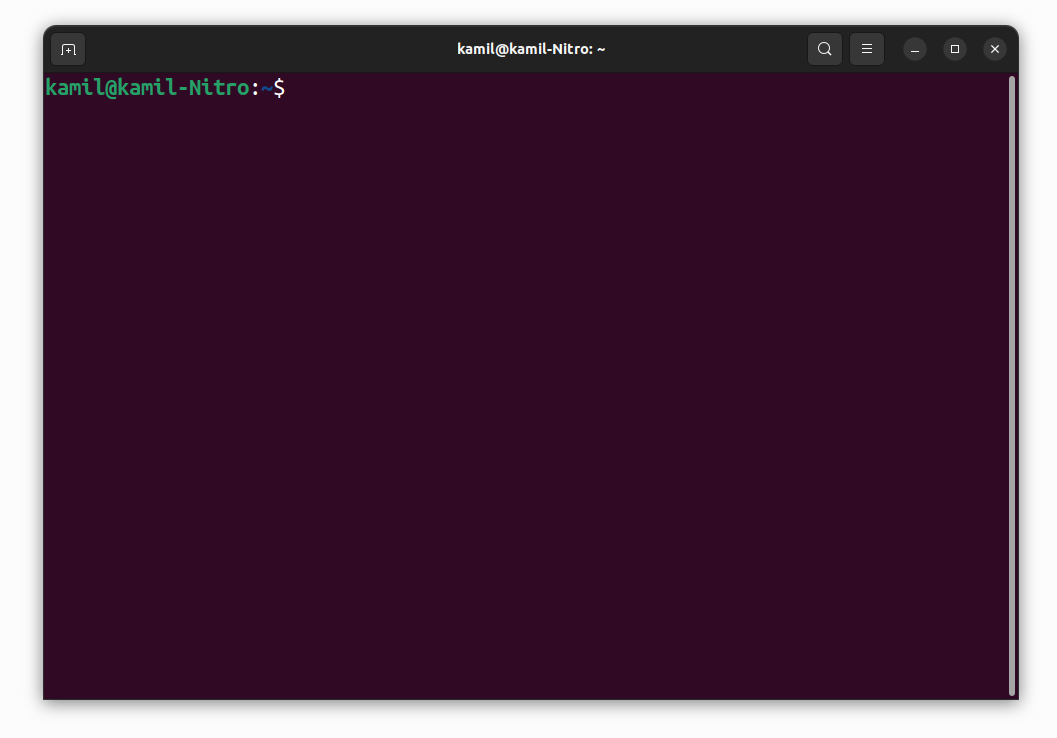
\includegraphics[scale=0.23]
    {./Presentations-pictures/Miscancellous-pictures/BASH-shell.png}


    \caption{Przykładowy wygląd włączonej powłoki \textsc{bash}, naszego
      głównego narzędzia pracy na tym przedmiocie.}


    \label{fig:BASH-shell}

  \end{figure}

\end{frame}
% ##################





% ##################
\begin{frame}
  \frametitle{Postęp technologiczny}

  \vspace{-0.5em}


  \begin{figure}

    \label{fig:Evolution-of-OS}

    \centering


    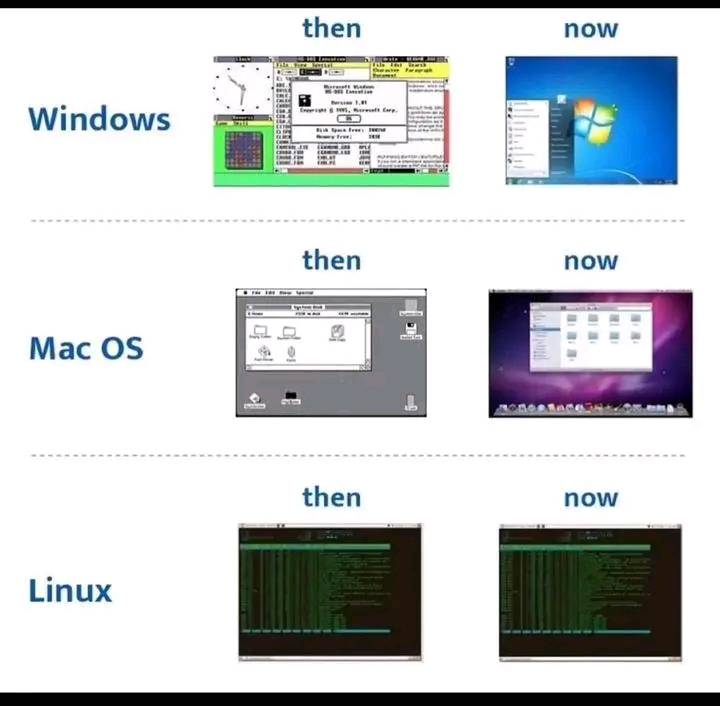
\includegraphics[scale=0.3]
    {./Presentations-pictures/Miscancellous-pictures/Evolution-of-operating-systems.jpg}

  \end{figure}

\end{frame}
% ##################





% ##################
\begin{frame}
  \frametitle{Włączanie powłoki}


  \textit{Gdy samochody rozwijały~się tak jak komputery, to dziś
    Rolls-Royce kosztowałby jakieś 100\$, przejeżdżałaby milion mil na
    jednym galonie benzyny i~raz do roku eksplodował zabijając wszystkich
    w~środku.} \\
  Robert Cringely, \textit{InfoWorld}, tłum. swobodne, str.~221,
  \parencite{Garfinkel-Weise-Strassmann-The-UNIX-HATERS-Handbook-Pub-1994}.


  Naszym główny narzędziem na tych zajęciach będzie powłoka
  (ang. \textit{shell}) \textsc{bash}, więc upewnijmy~się, że~umiemy ją
  włączyć, co na samy początku może być naprawdę niewdzięcznym zadaniem.
  W~pierwszym kroku proszę wcisnąć \texttt{Ctrl-Alt-t} i~zobaczyć, czy~się
  otworzy.

  Jeśli to nie zadziała, to proszę pochodzić kursorem po ekranie,
  aż~znajdziemy okienko „Szukaj”, „Wyszukaj” lub jeszcze jakaś inna nazwa.
  Proszę tam wpisać „Terminal”, „Konsola” lub „Consol” i~zobaczyć, czy
  wyświetli~się odpowiednia ikona.

  % !!!!!!! Nie usuwać.
  % Istnieje wiele wartych uwagi materiałów do nauki \textsc{bash}a, niekiedy
  % dość już wiekowych. Przykładowo, można sięgnąć do tutorialu
  % Gilesa Orra
  % \colorhref{https://www.gilesorr.com/bashprompt/howto/}
  % {\textit{Bash Prompt HOWTO}} \parencite{Orr-Bash-Prompt-HOWTO-Ver-2009}.

\end{frame}
% ##################





% ##################
\begin{frame}
  \frametitle{Architektura systemu operacyjnego}


  Pracując z~poziomu powłoki nie raz natkniemy~się na problemy
  trybów działania systemu operacyjnego oraz różnych poziomów dostępu.
  Często będzie to wynikiem przypadku i~możemy~się poczuć zagubienie,
  gdy przestanie działać w~zrozumiały sposób. Z~tego powodu wyjaśnimy teraz
  kilka pojęć dotyczących systemów operacyjnych.

  W~tym momencie potrzebujemy wprowadzić nowe pojęcie.
  \textbf{Architekturą systemu operacyjnego} nazywamy ogólny plan budowy
  danego systemu operacyjnego. Architektura takiego systemu jest więc
  zbiorem idei, których używamy do tworzenia oraz opisywania systemów
  operacyjnych. Jak poprzednio, nie będziemy potrzebowali ściślejszej
  definicji tego pojęcia.

\end{frame}
% ##################





% ##################
\begin{frame}
  \frametitle{Rola systemu operacyjnego}


  Podstawowa dziś architektura stosowana dzisiaj, mówi nam, że~system
  operacyjny może działać w~dwóch podstawowych trybach: trybie jądra
  i~trybie użytkownika. Oprócz tego dany system operacyjny może wprowadzać
  inne tryby i~poziomy dostępu, o~kilku z~nich powiemy później. Żeby
  zrozumieć czemu ten podział został wprowadzony, wróćmy do zagadnienia:
  po co istnieje system operacyjny?

  System operacyjny istnieje, by zdjąć z~nas obowiązek bezpośredniego
  zarządzania sprzętem, robienia takich rzeczy jak ręczne ustawienie
  wartości rejestrów procesora, od~których normalny użytkownik chce~się
  trzymać z~daleka. Oprócz tego, że~życie użytkownika staje~się przez to
  prostsze,
  to jest też bezpieczniejsze, bo pracując na niskim poziomie abstrakcji,
  łatwiej o~pomyłki i~poważne błędy. Przykładowo, potrzebuje mieć możliwość
  kasowania danych na dysku. Co jeśli przypadkiem zamiast usunąć jeden
  plik wydamy polecenie, by~skasować całą zawartość dysku?

\end{frame}
% ##################





% ##################
\begin{frame}
  \frametitle{Tryby działania systemu operacyjnego}


  Co więcej, jeśli kilka osób ma dostęp do tego samego komputera, to
  należy zagwarantować, żeby dane jednej osoby, które powinny pozostać
  tajne, nie były od ręki dostępne innym jego użytkownikom.

  Aby zapewnić możliwie dużą wygodę, bezpieczeństwo i~tajność danych,
  w~obecnej architekturze systemów operacyjnych dostępne są dwa główne tryby
  działania: \textbf{tryb jądra} (ang. \textit{kernel mode})
  i~\textbf{tryb użytkownika} (ang. \textit{user mode}). Należy pamiętać,
  że~to są dwa różne tryby działania tego samego programu.

  Pracując w~trybie jądra, możemy korzystać z~wszystkich możliwości jakie
  udostępnia nam sprzęt oraz mam dostęp do całej pamięci. Tryb ten musi
  istnieć, bo~wszystkie operacje sprzętu są potrzebne do działania
  komputera, więc
  ktoś musi mieć możliwość je uruchomić. Tak samo, ktoś musi mieć dostęp do
  całej pamięci, aby móc przydzielać ją innym.

\end{frame}
% ##################





% ##################
\begin{frame}
  \frametitle{Tryb użytkownika}


  Przejdźmy teraz do trybu użytkownika. Gdy jesteśmy w~tym trybie, system
  operacyjny wyłącza nam dostęp do pewny możliwości naszego komputera.
  W~szczególności, jeśli jakaś część pamięci jest przydzielona innemu
  użytkownikowi, jest ona dla nas niedostępna.

  Jak tego typu ograniczenia działają w~praktyce? System operacyjny jest
  programem jak każdy inny, więc jego działanie zależy od~ustawień. Jeśli
  działając jako użytkownik chcemy zobaczyć zawartość jakiegoś fragmentu
  pamięci, to wysyłamy zapytanie do systemu operacyjnego o~jej wyświetlenie
  nam. System, który zawsze widzi całą dostępną pamięć, sprawdza, czy ma
  prawo udostępnić nam ten konkretny fragment. Jeśli nie to przesyła nam
  wiadomość, że~nie mamy uprawnień do zobaczenia zawartości tej części
  pamięci.

  Więcej informacji w~temacie tych dwóch trybów działania można znaleźć
  w~tym wideo
  \parencite{Daves-Garage-Kernel-Mode-vs-User-Mode-Why-it-ETC-Ver-2024}.

\end{frame}
% ##################





% ##################
\begin{frame}
  \frametitle{Problemy z~bezpieczeństwem}


  Jak można~się z~tego domyślić, jeśli zdobędę dostęp do trybu jądra, mogę
  z~tym komputerem zrobić wszystko. Z~tego powodu hakerzy dokładają tylu
  starań, by uzyskać do niego dostęp \alert{bez} posiadania odpowiednich
  uprawnień. Dlatego też takie antycheaterskie programy takie jak Vanguard,
  który miał być dodany choćby do
  \colorhref{https://www.youtube.com/watch?v=nk6aKV2rY7E}{\textit{League~of
      Legends}}~są tak problematyczne
  \parencite{Low-Level-Why-Riots-anti-cheat-is-a-HUGE-problem-Ver-2024}.

  Vanguard działa bowiem w~trybie jądra, ma więc możliwość by zrobić
  z~moich komputerem absolutnie wszystko co chce. Czy ufamy firmie
  tworzącej ten program, że~nie nadużyje tych możliwości?

  Pytanie, czemu w~ogóle pozwalamy istnieć taki programom jak Vanguard?
  Dlatego, że~jeśli program ten pracuje w~trybie jądra to do wyszukiwania
  cheaterów używam zasobów \alert{naszych} komputera. Jeśli pracowałby
  w~trybie użytkownika, nie byłoby to możliwe, gdyż z~definicji trybu
  użytkownika, program ten nie miałby dostępu do informacji potrzebnych by
  wykryć cheatera.

\end{frame}
% ##################





% ##################
\begin{frame}
  \frametitle{Problemy z~bezpieczeństwem}


  Alternatywą jest uruchamianie tych programów na serwerze
  gry, który i~tak dysponuje wszystkimi tego typu informacjami. Co nie jest
  w~interesie firmy dostarczającej te serwery, dla niej jest lepiej jak
  serwery obsługują grę, a~wykrywaniem cheaterów zajmują~się komputery
  graczy.

\end{frame}
% ##################










% ######################################
\section{Pliki i~procesy}
% ######################################



% ##################
\begin{frame}
  \frametitle{Pliki i~procesy}


  Dwie podstawowe abstrakcje, których będziemy używać na tym kursie,
  to~\textbf{pliki} i~\textbf{procesy}. Nie wnikając w~szczegóły wystarczy
  nam stwierdzenie, że~plik czymś jest, a~proces coś robi. Warto tutaj
  przytoczyć następujące powiedzenie, które funkcjonuje w~wielu różnych
  wersjach i~różnych systemów operacyjnych.

  \textit{Wszystko w~systemie Linux jest plikiem. Jeśli coś nie jest
    plikiem to jest procesem.}

  Inaczej mówiąc, jeśli na komputerze znajdują~się jakieś dane, to są
  wewnątrz jakiegoś pliku. Jeśli komputer coś robi, to jest za to
  odpowiedzialny odpowiedni proces. Zrozumienie tego na tym poziomie jest
  wystarczające na~potrzeby tych zajęć. W~przyszłości może zajrzymy pod
  warstwę abstrakcji plików i~procesów, by~się przekonać, że~ich wewnętrzna
  budowa wcale nie jest banalna.

\end{frame}
% ##################





% ##################
\begin{frame}
  \frametitle{Pliki i~procesy}


  Ponieważ pliki są mniej abstrakcyjne (hehe), zaczniemy nasze zajęcia od
  zaznajomieniem~się z~pracą z~plikami pod powłoką \textsc{bash}.
  Przyjmujemy przy tym, że~znają Państwo pewne pojęcia z~systemu Windows.

\end{frame}
% ##################










% ######################################
\section{BASH nie zna słowa „litość”. Część~I}
% ######################################


% ##################
\begin{frame}
  \frametitle{Litość? Co to jest?}


  \textit{Gdy samochody rozwijały~się tak jak komputery, to dziś
    Rolls-Royce kosztowałby jakieś 100\$, przejeżdżałaby milion mil na
    jednym galonie benzyny i~raz do roku eksplodował zabijając wszystkich
    w~środku.} \\
  Robert Cringely, \textit{InfoWorld}, tłum. swobodne, str.~221,
  \parencite{Garfinkel-Weise-Strassmann-The-UNIX-HATERS-Handbook-Pub-1994}.

  Bóg jest litościwy, \textsc{bash} nie zna tego słowa. Przekonają~się
  Państwo o~tym wielokrotnie. Każdy z~nas popełnia literówki i~\textsc{bash}
  bez najmniejszej krztyny litości wytknie nam każdą z~nich, albo
  z~jej powodu zinterpretuje wszystko na~opak. Jak z~wieloma innymi
  rzeczami, trzeba nauczyć~się z~tym żyć.

  Kolejny problem dotyczy białych znaków (ang. \textit{whitespaces}), przy
  czym przez „białe znaki” rozumiemy wszystkie odstępy w~tekście, które na
  kartce papieru są po prostu obszarami bieli (albo innego koloru papieru).
  Trzy podstawowe białe znaki to spacja, tabulator i~znak nowej linii
  (klawisz \texttt{Enter}).

\end{frame}
% ##################





% ##################
\begin{frame}
  \frametitle{Swoboda używania białych znaków? Nie żartuj.}


  Języki takie jak~C, czy nawet Python dają nam dużą swobodę
  w~pisaniu białych znaków w~tekście. Wolność jaką mamy w~tym względzie
  w~\textsc{bash}u, to wolność do podróżowania jaką mam więzień zamknięty
  w~celi. Chodzi po celi można, ale czy to nazwiemy podróżą? Uczulam więc
  Państwa, na to by pilnować, gdzie są białe znaki. Jeśli coś
  w~\textsc{bash}u nie działa, to jest bardzo prawdopodobnie, iż~jest to
  wynik spacji w~złym miejscu.

  Będzie~się starali zaznaczać miejsca, gdzie szczególnie łatwo popełnić
  błąd, jednak podanie wszystkich zasada pisania w~\textsc{bash}u i~wyjątków
  od nich to naprawdę nie jest łatwa rzecz. Dlatego jeśli coś nie działa,
  to proszę sprawdzić, czy wpisane polecenia wyglądają \alert{dokładnie}
  tak jak zaprezentowane przykłady.

  Błędy w~przykładach też mogą~się zdarzać, prosimy by pisać o~nich do nas
  po adres \email.

\end{frame}
% ##################





% ##################
\begin{frame}
  \frametitle{Z~BASHem dzieje~się coś dziwnego}


  Błędne wprowadzenie jakiegoś polecenia może spowodować, że~\textsc{bash}
  przestanie reagować, lub będzie reagował zupełnie nie tak jak tego
  oczekujemy. Ponieważ \textsc{bash} nie wiem czym jest litość, w~zależności
  od tego co konkretnie~się zepsuło, dokładna procedura naprawy jest inna.

  Jednak w~większości przypadków, by wrócić do normalnej pracy wystarczy
  wcisnąć \alert{raz} \texttt{Ctrl-d}. Należy zaznaczyć, że~wciśnięcie
  \texttt{Ctrl-d} \alert{więcej niż raz} może spowodować zamknięcie powłoki
  \textsc{bash} i~potrzeby zrobienia kilku rzeczy ponownie. Z~tego też
  powodu, początkujący \alert{nigdy} nie powinni używać tego skrótu, jeśli
  wszystko działa jak trzeba.

  Mimo tych zastrzeżeń, \texttt{Ctrl-d} jest jednym z~naszych najlepszych
  przyjaciół.

\end{frame}
% ##################










% ######################################
\section{Podstawy pracy z~poziomu powłoki BASH}
% ######################################



% ##################
\begin{frame}
  \frametitle{Kilka słów wstępnych i~ostrzeżeń}


  Przed chwilą mówiliśmy, że~\textsc{bash} nie zna słowa litość i~każda
  drobna zmiana może wszystko zniszczyć. Jednocześnie nasza swoboda nie jest
  całkiem zerowa (choć może często sprawiać takie wrażenie), więc
  podając tutaj różne polecenia, musimy zdecydować~się na pewno konwencje.
  Proszę więc mieć świadomość, że~\alert{pewne} zmiany można wprowadzić
  do~poleceń i~nie zmienią one sposób ich działania.

  Jednak zasady które mówią co \alert{można} zmienić w~poleceniu
  \textsc{bash}a, bez obrócenia wszystkiego w~ruiny, są często nieintuicyjne
  i~skomplikowane. Ponieważ zaś zawsze $1000$ różnych rzeczy może zepsuć
  dane polecenie, zdecydowaliśmy, że~w~tym kursie będziemy starali~się
  podawać te wersje poleceń, które my uważamy za~optymalne i~które działają
  poprawnie, nie zaś wnikać w~pokrętne zasady „możesz zmienić to tak i~tak,
  ale~już nie w~ten sposób”.

\end{frame}
% ##################





% ##################
\begin{frame}
  \frametitle{Kilka słów wstępnych i~ostrzeżeń}


  Testowanie różnych wariantów tych poleceń, sprawdzanie który ich wariant
  działa, a~który nie, jest oczywiście czymś dobrym, co pozwala lepiej
  zrozumieć powłokę \textsc{bash}, więc bardzo nasz cieszy, gdy ktoś tego
  próbuje. Zajmuje to jednak czas, a~większość ludzi pragnie by „komputer
  zrobił to co trzeba”, nie zaś zgłębiać wszystkie niuanse jego pracy.
  Biorąc to wszystko pod uwagę, uznaliśmy, że~obecne sposób wykładu jest
  dobrym wyborem.

  Wszystko utrudnia dodatkowy fakt, że~od czasu do czasu można~się natknąć
  na~dwa warianty poleceń \textsc{bash}a, które działają tak samo, tylko,
  że~to nie do końca prawda. Działają tak samo w~$90\%$ przypadków,
  w~pozostały~$10\%$, działają inaczej. By uniknąć niekończących~się
  dywagacji na temat dzielenia włosa na czworo w~\textsc{bash}u, proszę
  przyjąć, że~jeśli polecenie nie działa jak trzeba, należy~się upewnić,
  iż~są one \alert{dokładnie} takie jak podano tutaj.

\end{frame}
% ##################





% ##################
\begin{frame}
  \frametitle{Kilka słów wstępnych i~ostrzeżeń}


  Do problemu, której wersji poleceń/kodu \textsc{bash}a należy używać,
  wrócimy jeszcze przy okazji pisania skryptów dla tej powłoki. To jednak
  na tą chwilę dość odległy temat.

  Pomimo tego, że~staramy~się dokładnie przetestować wszystkie podane
  w~tych wykładach polecenia \textsc{bash}a, nie możemy wykluczyć tego,
  że~popełnimy jakiś błąd. Dlatego bardzo prosimy by każdy, kto taki
  znajdzie, przesłał go nam pod adres \email.

\end{frame}
% ##################





% ##################
\begin{frame}
  \frametitle{Zaczynamy}


  Zacznijmy od przyjęcia, że~pracujemy na komputerze jako użytkownik,
  którego nazwa w~systemie operacyjnym została wybrana jako \texttt{adam}.
  Jeśli włączymy konsolę zobaczymy pewnie coś takiego: \\
  \texttt{adam:$\sim$\$} \\
  Od tego momentu będziemy zwykle skracali ten znak zachęty \\
  (ang.~\textit{prompt}) do symbolu \texttt{\$}. Przepisywanie pełnej jego
  postaci wnosi bardzo mało informacji, za~to zabiera sporo miejsca.

  Na początku zajmiemy~się tym, jak poruszać~się po systemie plików
  i~katalogów. Na pewno wiedzą Państwo, że~na komputerze znajdują~się
  katalogi (ang.~\textit{directories}), zwane też folderami, które zawierają
  pliki i~inne katalogi. Z~punktu widzenia systemu GNU/Linux
  katalog jest plikiem, jedynie specjalnego rodzaju. Dla tego systemu
  wszystko jest plikiem lub procesem.

\end{frame}
% ##################





% ##################
\begin{frame}
  \frametitle{Polecenia}


  Podstawy działania katalogów w~systemie GNU/Linux są w~zasadzie takie
  same jak w~systemie Windows, musimy~się jedynie przyzwyczaić do innych
  konwencji używanych w~tym systemie. Dużo większym wyzwaniem zapewne
  będzie zamienienie środowiska graficznego (\textsc{gui},
  ang.~\textit{Graphic User Interface}) na pracę z~poziomu powłoki.

  Podstawą pracy w~powłoce \textsc{bash} jest korzystanie z~poleceń (ang.
  \textit{commands}). Bez wnikania w~szczegóły, każde polecenie posiada
  nazwę i~wykonuje pewne działanie. By wykonać dane polecenie w~powłoce
  należy najpierw wpisać jej nazwę, następnie zaś jej odpowiednie
  opcje (flagi) i~argumenty. Część poleceń można wykonać bez wpisywania
  opcji czy~argumentów.

  Trzeba~się niestety przyzwyczaić do tego, że~nazwy poleceń, jak i~nazwy
  ich opcji tych poleceń w~systemie GNU/Linux potrafią być dość dziwne
  i~trudne do~zapamiętania.

\end{frame}
% ##################





% ##################
\begin{frame}
  \frametitle{Polecenia}


  Podstawowych poleceń systemu GNU/Linux jest około~$100$, do tego każde ma
  kilkanaście albo więcej opcji. Z~tego powodu nauka ich jest bardzo
  czasochłonna i~niełatwa. Teoretycznie w~każdej chwili w~\textsc{bash}u
  możemy skorzystać z~manuala (podręcznika), gdzie są opisy wszystkich
  poleceń. W~praktyce, żeby zrozumieć jego treść, wymagana jest już dość
  spora wiedza.

  Zdecydowaliśmy~się przyjąć następujące podejście. Naszym głównym celem
  jest przekazanie Państwu umiejętności pracy spod powłoki \textsc{bash}
  w~możliwie krótki i~bezbolesny sposób. Dlatego też, dość szybko
  wprowadzimy możliwie dużo poleceń, bez zagłębiania~się w~zbyt wiele
  szczegółów. Niekiedy będziemy wracać do wcześniej już omówionych poleceń,
  by uzupełnić wiadomości o~nich. Wyczerpujące omówienie wszystkich
  podstawowych poleceń i~tak zabrałoby zbyt dużo czasu, to zaś podejście
  uważamy, za rozsądny kompromis.

\end{frame}
% ##################





% ##################
\begin{frame}
  \frametitle{Polecenie \texttt{ls}}


  Zacznijmy od~polecenia
  \colorhref{https://linux.fandom.com/pl/wiki/Ls}{\texttt{ls}}. Jego nazwa
  pochodzi prawdopodobnie od~ang.~\textit{List fileS}, ale są różne opinie
  na ten temat. Polecenie to wyświetla zawartość katalogu w~którym~się
  znajdujemy, z~tego powodu wynik działania tego polecenia będzie~się cały
  czas zmieniać, jednym z~możliwych może być ten przedstawiony poniżej. \\
  \texttt{\$ ls} \\
  \texttt{{\color{jAxisBlue} Dokumenty}} \quad
  \texttt{introduction-to-GNU-linux.pdf} \quad
  \texttt{{\color{jAxisBlue} Pobrane}}

  Polecenie \texttt{ls} jest przykładem takiego polecenia, które można
  uruchomić bez dodatkowych opcji czy argumentów, ono samo ustali w~jakim
  katalogu jesteśmy i~wypisze jego zawartość.

  Obecnie jest standardem, że~powłoka używa kolorów i~różnych typów fontów,
  by~informować nas o~typie i~własnościach pliku. W~przykładzie powyżej
  nazwy katalogów są wyróżnione na niebiesko, trzeba jednak pamiętać,
  że~wszystko to~zależy od~konkretnych ustawień systemu operacyjnego
  i~łatwo może zostać zmienione.

\end{frame}
% ##################





% ##################
\begin{frame}
  \frametitle{Polecenie \texttt{pwd}}


  Kolejnym poleceniem jest
  \colorhref{https://www.arturpyszczuk.pl/commands-pwd.html}{\texttt{pwd}}
  od ang.~\textit{Print Working Directory}, rezultat jego działania można
  zobaczyć poniżej. \\
  \texttt{\$ pwd} \\
  \texttt{/home/adam}

  Ta krótka linia zawiera bardzo dużo informacji i~potrzebujemy przynajmniej
  kilka z~nich wyjaśnić. Sposób w~jaki pliki i~katalogi są ułożone na~dysku
  jest zdefiniowane przez \textbf{system plików} danego systemu
  operacyjnego i~ten używany w~systemie GNU/Linux różni~się mocno tego
  w~systemie Windows.

  Zacznijmy od kilku uwag odnośnie notacji. Jeśli pracowalibyśmy w~tym
  ostatnim systemie i~na dysku~C znajdowałby~się
  katalog \texttt{Systemy-operacyjne-Ćwiczenia} a~w~nim katalog
  \texttt{Zajęcia-01}, to ścieżka do niego miałaby postać: \\
  \texttt{C:\textbackslash\textbackslash
    Systemy-operacyjne-Ćwiczenia\textbackslash Zajęcia-01} \\

\end{frame}
% ##################





% ##################
\begin{frame}
  \frametitle{System plików}


  Odpowiednikiem ścieżki z~systemu Windows: \\
  \texttt{C:\textbackslash\textbackslash
    Systemy-operacyjne-Ćwiczenia\textbackslash Zajęcia-01} \\
  w~systemie GNU/Linux byłaby ścieżka: \\
  \texttt{/home/adam/Systemy-operacyjne-Ćwiczenia/Zajęcia-01} \\
  Widzimy więc, że~gdy Windows do oddzielania nazw katalogów i~plików
  używa symbolu „backslasha”: „\texttt{\textbackslash}”, to GNU/Linux
  używa symbolu „slasha”: „\texttt{/}”. Jest to stosunkowo mała różnica,
  ale trzeba~się do niej przyzwyczaić.

  Poważniejsza różnica jest następująca. Komputery z~systemem GNU/Linux
  mogą posiadać wiele dysków, nie jest to żadnym problemem, ale~system
  plików GNU/Linuxa nie zna pojęcia dysku jako takiego. W~systemie GNU/Linux
  istnienie naczelny katalog zwany rootem, czyli po polsku „korzeniem”,
  w~którym zawierając~się wszystkie inne pliki oraz katalogi, nieważne na
  którym fizycznym dysku są one umieszczone. Katalog root oznaczamy
  symbolem~„\texttt{/}”.

\end{frame}
% ##################





% % ##################
% \begin{frame}
%   \frametitle{System plików}


%   Odpowiednikiem ścieżki z~systemu Windows: \\
%   \texttt{C:\textbackslash\textbackslash
%     Systemy-operacyjne-Ćwiczenia\textbackslash Zajęcia-01} \\
%   w~systemie GNU/Linux byłaby ścieżka: \\
%   \texttt{/home/adam/Systemy-operacyjne-Ćwiczenia/Zajęcia-01} \\
%   Widzimy więc, że~gdy Windows do oddzielania nazw katalogów i~plików
%   używa symbolu „backslasha”: „\texttt{\textbackslash}”, to GNU/Linux
%   używa symbolu „slasha”: „\texttt{/}”. Jest to stosunkowo mała różnica,
%   ale trzeba~się do niej przyzwyczaić.

%   Poważniejsza różnica jest następująca. Komputery z~systemem GNU/Linux
%   mogą posiadać wiele dysków, nie jest to żadnym problemem, ale~system
%   plików GNU/Linuxa nie zna pojęcia dysku jako takiego. W~systemie GNU/Linux
%   istnienie naczelny katalog zwany rootem, czyli po polsku „korzeniem”,
%   w~którym zawierając~się wszystkie inne pliki oraz katalogi, nieważne na
%   którym fizycznym dysku są one umieszczone. Katalog root oznaczamy
%   symbolem~„\texttt{/}”.

% \end{frame}
% % ##################





% ##################
\begin{frame}
  \frametitle{System plików}


  Wróćmy do polecenia \\
  \texttt{\$ pwd} \\
  \texttt{/home/adam} \\
  Linię \texttt{/home/adam} czytamy „W~katalogu root („\texttt{/}”)
  znajduje~się katalog \texttt{home}, w~nim zaś znajduje~się katalog
  \texttt{adam}.” Polecenie \texttt{pwd} podaje więc w~którym katalogu~się
  obecnie znajdujemy, za~pomocą ścieżki, która zaczyna~się od katalogu root:
  „\texttt{/}”.

  Katalog w~którym obecnie jesteśmy nosi nazwę \textbf{katalogu roboczego}
  (ang.~\textit{working directory}), a~jak powiedzieliśmy \texttt{pwd} jest
  akronimem od~\textit{Print Working Directory}, czyli „wyświetl katalog
  roboczy”.

  Ścieżkę podającą lokalizację katalogu lub pliku nazywamy
  \textbf{ścieżką bezwzględną}, jeśli zaczyna~się ona od katalogu root.
  W~przeciwnym razie mówimy o~\textbf{ścieżce względnej} (podawanej
  względem innego katalogu niż root).

\end{frame}
% ##################





% ##################
\begin{frame}
  \frametitle{System plików}


  Bez wielkich uproszczeń można przyjąć, że~\textsc{bash}u \alert{każdy}
  ciąg symboli zaczynający od~symbolu „\texttt{/}” zostanie zinterpretowany
  jako ścieżka do jakiegoś pliku lub katalogu. Z~tego powodu trzeba
  \alert{bardzo} uważać przy stosowaniu symbolu~„\texttt{/}”.

  W~szczególności, gdy stosujemy symbol „\texttt{/}”, trzeba zwracać dużą
  uwagę na~spacje. Ścieżka postaci \\
  \texttt{/home/adam} \\
  jest poprawna. Ale już ścieżka \\
  \texttt{/ home/adam} \\
  jest \alert{błędna}! To w~jaki sposób jest błędna, to omówimy innym
  razem. Doświadczenie uczy, że~na początku sprawia to ludziom
  bardzo dużo problemów.

  To, że~główny katalog nosi nazwę „korzenia” (ang.~\textit{root}) nie jest
  przypadkiem, ale do tej kwestii wrócimy innym razem.

\end{frame}
% ##################





% ##################
\begin{frame}
  \frametitle{Katalog domowy}


  W~systemie GNU/Linux każdy użytkownik ma swój katalog domowy, w~którym
  może przechowywać potrzebne mu pliki. Standardowo, choć mogą być wyjątki,
  użytkownik \texttt{adam} otrzyma katalog \texttt{/home/adam}, użytkownik
  \texttt{barbara} katalog \texttt{/home/barbara},~etc. Katalog domowy
  bieżącego użytkownika posiada też alternatywną nazwę „$\sim$”. Stąd znak
  zachęty \\
  \texttt{adam:$\sim$\$} \\
  przekazuje nam informację, że~działamy jako użytkownik \texttt{adam}
  i~znajdujemy~się w~jego katalogu domowym.

  Załóżmy, że~katalogu domowym znajduje~się katalog o~nazwie
  \texttt{Systemy-operacyjne-Ćwiczenia}. By sprawdzić, czy tak jest
  naprawdę możemy użyć polecenia \texttt{ls}: \\
  \texttt{\$ ls} \\
  \texttt{{\color{jAxisBlue} Dokumenty}} \quad
  \texttt{introduction-to-GNU-linux.pdf} \quad
  \texttt{{\color{jAxisBlue} Pobrane}} \\
  \texttt{{\color{jAxisBlue} Systemy-operacyjne-Ćwiczenia}} \\

\end{frame}
% ##################





% ##################
\begin{frame}
  \frametitle{Polecenie \texttt{cd}}


  Jeśli w~bieżącym katalogu znajduje~się katalog
  \texttt{Systemy-operacyjne-Ćwiczenia} to możemy do niego wejść
  używając polecenia
  \colorhref{https://linux.fandom.com/pl/wiki/Cd}{\texttt{cd}}
  (od ang.~\textit{Change Directory}): \\
  \texttt{adam:$\sim$\$ cd Systemy-operacyjne-Ćwiczenia} \\
  \texttt{adam:$\sim$/Systemy-operacyjne-Ćwiczenia\$} \\
  Wyjątkowo zapisaliśmy pełniejszą wersję znaku zachęty, by podkreślić,
  iż~informuje on~nas w~którym katalogu jesteśmy. Mianowicie ścieżka
  \texttt{$\sim$/Systemy-operacyjne-Ćwiczenia} informuje nas, że~w~katalogu
  domowych użytkownika \texttt{adam} znajduje~się katalog
  \texttt{Systemy-operacyjne-Ćwiczenia} i~w~nim właśnie jesteśmy.

  Użyte wyżej polecenie \texttt{cd} jest przykładem polecenia, które
  pobiera argument, mianowicie nazwę katalogu do którego możemy wejść.
  W~istocie polecenie to pozwala nam na bardzo swobodne poruszanie~się
  po systemie plików, jeśli opanujemy dobrze zapis ścieżek w~GNU/Linuxie,
  ale wszystko po kolei.

\end{frame}
% ##################





% ##################
\begin{frame}
  \frametitle{Polecenie \texttt{cd}}


  Załóżmy, że~teraz chcielibyśmy przejść do katalogu nad nami. By to zrobić
  należy przekazać poleceniu \texttt{cd} argument „\texttt{..}”: \\
  \texttt{adam:$\sim$/Systemy-operacyjne-Ćwiczenia\$ cd ..} \\
  \texttt{adam:$\sim$\$} \\
  Dlaczego jako argument przesyłamy akurat „\texttt{..}” wyjaśnimy w~swoim
  czasie, na razie przyjmijmy, iż~tak po prostu jest. Dla lepszej
  ilustracji tego co~zrobiliśmy, ponownie wypisaliśmy znak zachęty,

  Załóżmy, że~chcemy teraz wejść do katalogu
  \texttt{Systemy-operacyjne-Ćwiczenia} i~utworzyć tam plik
  \texttt{Notatki-z-zajęć.txt}. By utworzyć ten plik możemy skorzystać
  z~polecenia
  \colorhref{https://linux.fandom.com/pl/wiki/Touch}{\texttt{touch}}. Pełna
  sekwencja poleceń będzie wyglądać tak. \\
  \texttt{\$ cd Systemy-operacyjne-Ćwiczenia} \\
  \texttt{\$ touch Notatki-z-zajęć.txt} \\

\end{frame}
% ##################





% ##################
\begin{frame}
  \frametitle{Edycja plików z~pomocą programu gedit}


  Możemy teraz użyć polecenia \texttt{ls} by~się przekonać, czy~plik
  \texttt{Notatki-z-zajęć.txt} został poprawnie utworzony.
  Z~komputerami nigdy nic nie wiadomo, więc warto to sprawdzić.

  W~następnym kroku otworzymy go do edycji za~pomocą programu
  \colorhref{https://gedit-text-editor.org/}{gedit}. By to zrobić
  wpisujemy w~powłoce \\
  \texttt{\$ gedit Notatki-z-zajęć.txt \&} \\
  Proszę pamiętać o~dodaniu na końcu polecenia znaku
  \alert{ampersand}:~„\&”. Inaczej gedit zablokuje nam możliwość wpisywania
  kolejnych poleceń do powłoki i~by ją odzyskać, będziemy musieli
  wyłączyć gedita albo użyć kombinacji poleceń \texttt{jobs} i~\texttt{bg}.

  Czemu uruchomienie gedita bez symbolu ampersanda ma takie skutki, omówimy
  gdy będziemy dyskutowali zagadnienie procesów i~tego jak działają
  w~systemie GNU/Linux. Nie jest to najprostszy temat na świecie.

\end{frame}
% ##################





% ##################
\begin{frame}
  \frametitle{Okienko gedita}


  Jeśli wszystko poszło dobrze, to na ekranie zobaczymy okienko Gedita,
  które wygląda mniej więcej tak jak to na~zdjęciu~\eqref{fig:Gedit-window}.





  \begin{figure}

    \centering

    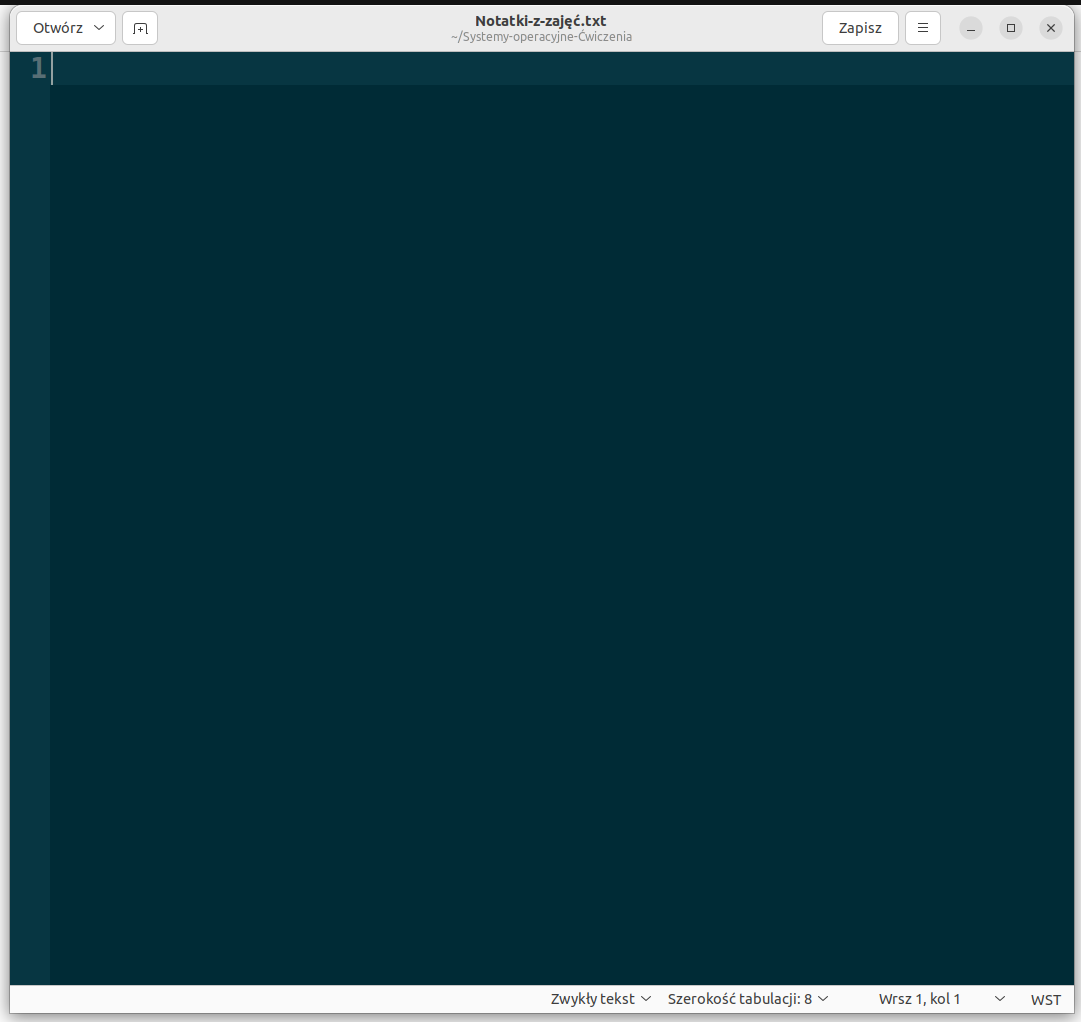
\includegraphics[scale=0.145]
    {./Presentations-pictures/Miscancellous-pictures/gedit-window.png}

    \caption{Otwarte okienko programu gedit.}


    \label{fig:Gedit-window}

  \end{figure}

\end{frame}
% ##################





% ##################
\begin{frame}
  \frametitle{Edytory tekstów}


  Teraz możemy do pliku \texttt{Notatki-z-zajęć.txt} wpisać tekst, choćby
  \textit{Notatki z~przedmiotu „Systemy operacyjne”}. Proszę pamiętać, by
  zapisywać wprowadzone zmiany, służy do tego choćby skrót~\texttt{Ctrl-s}.

  Kilka słów dlaczego wybraliśmy do~edycji plików program gedit. Na~tym
  kursie korzystamy głównie z~niego, gdyż jest on prosty w~obsłudze
  i~w~kilka sekund po jego otwarciu użytkownik może już pisać odpowiedni
  tekst. Zostawiamy jednak Państwu pełną swobodę w~wyborze edytora tekstu.
  Nie jest ważne jakiego programu~się używa, ważne jest, żeby udało~się
  wykonać zadanie jakie przed nami stoi.

  Jeśli chodzi o~edytory dostępne pod systemem GNU/Linux, to w~naszej
  ocenie warto zwrócić uwagę choćby na~dwa owiane już legendą programy
  do edycji tekstu \colorhref{https://www.vim.org/}{vim}
  i~\colorhref{https://www.gnu.org/software/emacs/}{GNU Emacs}.

\end{frame}
% ##################










% ######################################
\section{Dalsze informacje o~pracy z~BASHem}
% ######################################


% ##################
\begin{frame}
  \frametitle{Pewne subtelności}


  Przyjmijmy, że~jesteśmy w~katalogu \texttt{Systemy-operacyjne-Ćwiczenia}
  i~mamy utworzony plik \texttt{Notatki-z-zajęć.txt}. Każdy system
  operacyjny musi podjąć decyzję, czy traktuje on duże i~małe litery
  jako różne symbole, czy jako dwie wersje tego samego symbolu. Problem
  sprowadza~się do tego, czy \texttt{Notatki-z-zajęć.txt}
  i~\texttt{notatki-z-zajęć.txt} są dwoma różnymi nazwami tego samego pliku,
  czy też są to dwie różne nazwy? Kwestia ta jest sprawą konwencji,
  ale~należy ją rozstrzygnąć by uniknąć nieporozumień.

  Symbol GNU/Linux przyjął, że~duże i~małe litery to \alert{różne} symbole,
  więc \texttt{Notatki-z-zajęć.txt} i~\texttt{notatki-z-zajęć.txt} to dwie
  różne nazwy. Tak jak w~systemie Windows, w~systemie GNU/Linux w~danym
  katalogu może być tylko jeden plik o~danej nazwie. Jest to rozsądny wybór,
  gdyż inaczej użytkownik łatwo by~się pogubił.

\end{frame}
% ##################





% ##################
\begin{frame}
  \frametitle{Polecenie \texttt{mkdir}}


  Na mocy tego co powiedzieliśmy wyżej, w~tym samym katalogu mogą
  współistnieć pliki o~nazwie \texttt{Notatki-z-zajęć.txt}
  i~\texttt{notatki-z-zajęć.txt}. Byłyby to \alert{różne} pliki, zawartość
  jednego z~nich nie miałaby nic wspólnego z~zawartością drugiego. Jednak
  by uniknąć bałaganu, należy unikać podobnych nazw plików.

  Powiedzmy, że~chcemy teraz utworzyć w~naszym katalogu
  (\texttt{Systemy-operacyjne-Ćwiczenia}) katalog \texttt{Zajęcia-01}.
  Służy do tego polecenie
  \colorhref{https://www.arturpyszczuk.pl/commands-mkdir.html}
  {\texttt{mkdir}}. Polecenie to wymaga do działania argumentu, którym
  jest nazwa katalogu, który ma zostać utworzony (logiczne): \\
  \texttt{\$ mkdir Zajęcia-01} \\
  \texttt{\$ ls} \\
  \directoryName{Zajęcia-01} \quad \texttt{Notatki-z-zajęć.txt} \\
  Powiedzmy, że~stwierdziliśmy, że~chcemy zmienić nazwę pliku
  \texttt{Notatki-z-zajęć.txt} na
  \texttt{Notatki-z-systemów-operacyjnych-01.txt} i~przenieść do katalogu
  \texttt{Zajęcia-01}.

\end{frame}
% ##################





% ##################
\begin{frame}
  \frametitle{Polecenie \texttt{mv}}


  W~systemie GNU/Linux zarówno do zmiany nazwy pliku, jak i~przenoszenia
  ich między katalogami służy polecenie
  \colorhref{https://www.geeksforgeeks.org/mv-command-linux-examples/}
  {\texttt{mv}} (ang.~\textit{MoVe}). Możemy więc zmienić nazwę pliku
  za~pomocą polecenia: \\
  \texttt{\$ mv Notatki-z-zajęć.txt Notatki-z-systemów-operacyjnych-01.txt}

  Następnie możemy przenieść plik
  \texttt{Notatki-z-systemów-operacyjnych-01.txt} go do katalogu
  \texttt{Zajęcia-01} za pomocą polecenia: \\
  \texttt{\$ mv Notatki-z-systemów-operacyjnych-01.txt Zajęcia-01/} \\
  Symbol „\texttt{/}” na końcu nazwy katalogu nie jest niezbędny,
  ale~dobrze go tam umieszczać, bo~stanowi dodatkową informację
  dla~\textsc{bash}a i~użytkownika, że~konkretna nazwa jest nazwą
  katalogu.

  Ogólnie unikanie wszelkich niejednoznaczności jest dobrą praktyką.
  Dlatego dobrze jest w~ramach możliwości, jawnie zaznaczać charakter
  wszystkich bytów, występujących w~poleceniach.

\end{frame}
% ##################





% ##################
\begin{frame}
  \frametitle{Polecenie \texttt{mv}}


  Możemy też przenieść plik do katalogu i~zmienić jego nazwę za pomocą
  pojedynczego polecenia: \\
  \texttt{\$ mv Notatki-z-zajęć.txt
    Zajęcia-01/Notatki-z-systemów-operacyjnych-01.txt} \\
  Ponieważ polecenie \texttt{mv} może przenosić pliki tylko do istniejących
  już katalogów, samo potrafi wykryć co jest nazwą katalogu, a~co nową
  nazwą pliku. Jak z~większością poleceń GNU/Linuxa należy jednak unikać
  ich użycia, jeśli nie jesteśmy pewni co dane polecenie zrobi.

  Wszyscy zapewne dobrze wiemy, że w~systemie Windows, jeśli chcemy
  przekopiować plik o~nazwie \texttt{Dane.dat} do katalogu, który już
  zawiera plik o~tej nazwie, to zobaczymy komunikat typu
  \textit{Plik „Dane.dat” zostanie nadpisany. Czy chcesz kontynuować?}
  Niestety, to \alert{nie} jest domyślne działanie polecenia \texttt{mv}
  i~wielu innych poleceń w~systemie GNU/Linux.

\end{frame}
% ##################





% ##################
\begin{frame}
  \frametitle{Zagrożenia jakie stwarza \texttt{mv}}


  Załóżmy więc, że~jesteśmy w~katalogu w~którym znajduje~się plik
  \texttt{Ważne-dane.dat} i~plik \texttt{Tekst-popularnych-piosenek.txt}.
  Jeśli przez przypadek wprowadzimy polecenie \\
  \texttt{\$ mv Teksty-popularnych-piosenek.txt Ważne-dane.dat} \\
  to plik \texttt{Ważne-dane.dat} zostanie nadpisany przez niezbyt ważny
  plik \texttt{Teksty-popularnych-piosenek.txt}. Odzyskanie pliku
  \texttt{Ważne-dane.dat} nie jest niemożliwe, ale jest bardzo, ale to
  \alert{bardzo} trudne i~wymaga sporych umiejętności pracy z~systemem
  GNU/Linux.

  \textit{Jesteś prawdziwym miłośnikiem ryzyka, jeśli przechowujesz ważne
    pliki na~komputerze z~systemem \textsc{unix}.} \\
  Robert E.~Seastrom, tłum. swobodne, str.~$261$
  \parencite{Garfinkel-Weise-Strassmann-The-UNIX-HATERS-Handbook-Pub-1994}.
  Stwierdzenie to odnosi~się też do systemu GNU/Linux.

  Pomimo tych problemów, polecenia takie jak \texttt{mv} są zbyt ważne,
  by~ich nie używać. Jak~się jednak zabezpieczyć przed takimi problemami?

\end{frame}
% ##################





% ##################
\begin{frame}
  \frametitle{Jak rozsądnie korzystać z~\texttt{mv}?}


  Poprzez dodanie odpowiednich opcji (flag) do~polecenia \texttt{mv}
  może sprawić, że~zawsze, gdy polecenie to nadpisałoby istniejący
  plik zostaniemy zapytani, czy naprawdę chcielibyśmy to zrobić.
  W~tym przypadku opcja tą jest \texttt{-i}, rezultat jej działania
  przedstawiony jest poniżej. \\
  \texttt{\$ mv -i Teksty-popularnych-piosenek.txt Ważne-dane.dat} \\
  \texttt{mv: zamazać 'Ważne-dane.dat'?} \\
  Forma pytania jaką otrzymamy może być inna na Państwa komputerze.
  Odpowiedzi twierdzącej na to pytanie, możemy udzielić wpisując
  „\texttt{t}”, „\texttt{tak}”, „\texttt{y}” lub „\texttt{yes}”, wówczas
  plik \texttt{Ważne-dane.dat} zostanie nadpisany. Jeśli chcemy udzielić
  odpowiedzi przeczącej możemy wpisać „\texttt{n}”, „\texttt{nie}”
  lub~„\texttt{no}”.

  Opcje, jak sama nazwa wskazuje, zmieniają działanie polecenia i~na tym
  kursie nie musimy wiedzieć o~nich wiele więcej.

\end{frame}
% ##################





% ##################
\begin{frame}
  \frametitle{Opcje (flagi)}


  Ponieważ istnieje duże ryzyko, że~osoby rozpoczynają swoją przygodę
  z~powłoką nadpiszą przez przypadek ważny plik stosując polecenie
  \texttt{mv}, we wszystkich przykładach będziemy do niego dodawali
  opcję~\texttt{-i}. Wyjątkiem od tej zasady będą sytuacja, gdy chcemy
  by~polecenie \texttt{mv} nadpisało już istniejący plik.

  Doświadczeni użytkownicy systemu GNU/Linux już parokrotnie stracili ważne
  dane przez niewłaściwe użycie polecenia~\texttt{mv}, więc używają go
  znacznie ostrożniej i~przez to ryzyko utraty kolejnych danych tą metodą
  jest znacznie mniejsze.

  Opcje poleceń takie jak~\texttt{-i} mogą wyglądać dziwnie i~być ciężkie
  do zapamiętania, niestety, musimy nauczyć~się z~tym żyć. Ich poznawanie
  nie należy do przyjemnych, wymaga dużo zapamiętywania, częstego
  googlowania lub~nabycie umiejętności czytania trudnego w~zrozumieniu
  manuala (\texttt{man}). Do tego tematu jeszcze nie raz wrócimy.

\end{frame}
% ##################





% ##################
\begin{frame}
  \frametitle{Czemu życie nie może być proste?}


  Wszystkie te problemy nie zmieniają faktu, że~polecenia dostępne
  w~\textsc{bash}u wraz z~ich opcjami dają nam bardzo potężne narzędzie
  do~ręki i~ich poznanie jest niezbędne, jeśli chcemy naprawdę dobrze
  poznać system operacyjny GNU/Linux.

  O~opcjach różnych poleceń i~ich pokręconej logice powiemy sobie więcej
  podczas następnych spotkań.

\end{frame}
% ##################










% ######################################
\section{BASH nie zna słowa „litość”. Część~II}
% ######################################


% ##################
\begin{frame}
  \frametitle{Litość? Jaka litość?}


  Powłoka \textsc{bash} nie zna słowa litość. Powiedzmy, że~chcemy
  zmienić nazwę pliku \texttt{Data-01.dat} na \texttt{Data-January-04.dat}
  i~wpisujemy polecenie: \\
  \texttt{\$ mv - i Data-01.dat Data-January-04.dat} \\
  Wciskamy klawisz \texttt{Enter} i~widzimy coś takiego: \\
  \texttt{mv: cel 'Data-January-04.dat nie jest katalogiem} \\
  I~w~naszej głowie pojawia~się pytanie „Co~się dzieje?” Od razu zauważmy,
  że~na Państwa komputerach treść otrzymanego komunikatu może być inna.
  Problemowi okazuje~się być winna jest temu jedna, jedyna spacja między
  symbolem „\texttt{-}” oraz~„\texttt{i}”.

  Jeśli opcja zaczyna~się symbolem „\texttt{-}” to po nim
  \alert{nie może być spacji}! Poprawna wersja tego polecenia to \\
  \texttt{\$ mv -i Data-01.dat Data-January-04.dat}

  Jak~się zapewne już Państwo domyślają, istnieją opcje poleceń nie
  zaczynające~się od symbolu „\texttt{-}”, o~nich opowiemy sobie później.

\end{frame}
% ##################





% ##################
\begin{frame}
  \frametitle{Logika BASHa? Jaka logika?}


  Problem bierze~się stąd, że~jeśli wprowadzimy niepoprawne polecenie
  \texttt{\$ mv - i Data-01.dat Data-January-04.dat} \\
  to \textsc{bash} zinterpretuje „\texttt{-}”, „\texttt{i}” oraz
  „\texttt{Data-01.dat}” jako nazwy \alert{plików}, które ma przenieść
  do katalogu o~nazwie „\texttt{Data-January-04.dat}” i~zgłasza problem,
  że~plik \texttt{Data-January-04.dat} nie jest katalogiem.

  Polecenie \texttt{mv} zostało w~taki sposób napisane, że~oczekuje,
  iż~przesłana do niej opcja zaczyna~się od symbolu „\texttt{-}”,
  a~natychmiast po tym symbolu litera oznaczająca konkretną opcję.
  W~przeciwnym razie zinterpretuje następujące po nim napisy jako nazwy
  odpowiednich plików lub katalogów i~spróbuje wykonać na nich odpowiednią
  operację.

  Jak~się zapewne już Państwo domyślają, istnieją opcje poleceń nie
  zaczynające~się od symbolu „\texttt{-}”, o~nich opowiemy sobie później.

  Musimy podkreślić, że~w~tym co napisaliśmy jest wiele uproszczeń,
  ale~nie chcieliśmy wchodzić teraz w~zbyt wiele szczegółów.

\end{frame}
% ##################





% ##################
\begin{frame}
  \frametitle{Polecenia też ktoś napisał}


  Proszę pamiętać, że~polecenie \texttt{mv} jest programem, napisanym
  prawdopodobnie w~języku~C, który jakiś programista kiedyś stworzył i~ten
  człowiek zdecydował, że~to polecenie ma działać tak, a~nie inaczej.
  Często nie należy~się doszukiwać zbyt wiele logiki w~działaniu poleceń,
  one są takie, bo~tak po prostu wyszło.

  Gdybyśmy dziś tworzyli jakiś system operacyjny i~jego powłokę „od zera”,
  to pewnie byśmy zaprojektowali je inaczej. Trzeba wszak uczyć~się na
  własnych błędach ;).

\end{frame}
% ##################










% ######################################
\appendix
% ######################################





% ######################################
\EndingSlide{Dziękuję! Pytania?}
% ######################################










% ######################################
\section{Dlaczego BASH~się tak nazywa}
% ######################################



% ##################
\begin{frame}
  \frametitle{Dlaczego BASH~się tak nazywa?}


  Historia zaczyna~się
  od~\colorhref{https://en.wikipedia.org/wiki/Stephen\_R.\_Bourne}
  {Steve Bourne’a}, który w~$1979$~roku napisał powłokę, która w~naturalny
  sposób została nazwana
  \colorhref{https://en.wikipedia.org/wiki/Bourne\_shell}{powłoką Bourne’a}
  (ang.~\textit{Bourne shell}). Bazując na niej
  \colorhref{https://en.wikipedia.org/wiki/Brian\_Fox\_(programmer)}
  {Brian Jhan Fox} napisał w~$1989$~roku \textit{Bourne Again SHell},
  czyli właśnie
  \colorhref{https://en.wikipedia.org/wiki/Bash\_(Unix\_shell)}
  {\textsc{bash}a}.

  Sama nazwa \textit{Bourne again shell} to również żart językowy. Nazwę tę
  można bowiem przetłumaczyć jako „ponownie powłoka Borne’a”, jak
  i~„odrodzona na nowo powłoka”. W~tym drugim przypadku mamy do czynienia
  z~grą słowną z~terminem
  \colorhref{https://billygraham.org/answers/what-is-your-definition-of-a-born-again-christian}
  {\textit{being born again}}, który zyskał
  duże znaczenie teologiczne wśród protestantów z~nurtu
  \colorhref{https://pl.wikipedia.org/wiki/Ewangelikalizm}{ewangelikanizmu}.

\end{frame}
% ##################





% % ##################
% \jagiellonianendslide{?????}
% % ##################










% ####################################################################
% ####################################################################
% Bibliography

\printbibliography





% ####################################################################
% End of the document

\end{document}
